\hypertarget{objetivo-geral}{%
\section{Objetivo Geral}\label{objetivo-geral}}

O objetivo geral da parceria foi constituir a rede de laboratórios de
pesquisa e desenvolvimento de tecnologias inovadoras para políticas
públicas do Ministério da Cultura. O principal objetivo é pesquisar e
aplicar técnicas, metodologias de desenvolvimento de software, além de
aferição qualidade produto de software, em ambiente experimental do
Laboratório Avançado de Pesquisa, Produção e Inovação em Software
(LAPPIS). Tais pesquisas e práticas serão usadas para subsidiar o
Ministério da Cultura de ferramentas de gestão e desenvolvimento de
software colaborativo, aberto e contínuo, em diferentes arranjos
produtivos, aprimorando os mecanismos de governança digital; além de
fornecer subsídios tecnológicos que apoiem a execução da Lei 8.313/91,
conhecida como Rouanet e das demais políticas de fomento e incentivo a
cultura.

O presente relatório apresenta o acompanhamento do trabalho realizado no
projeto ``Ecossistemas de Software Livre'', Termo de Cooperação para
Descentralização de Crédito, Processo Ofício No 0646/2017/FUB-UnB,
Vigência Outubro 2017 a Outubro 2019. O relatório apresentado é
relatório final do projeto e vai apresentar o que foi realizado no
âmbito do projeto, os principais resultados, e entregas, a partir das
expectativas do plano de trabalho vigente.

\hypertarget{objetivos-especuxedficos}{%
\section{Objetivos Específicos}\label{objetivos-especuxedficos}}

No plano de trabalho foram levantados alguns objetivos específicos
referentes a parceria. Ao longo do relatório de entrega final serão
detalhadas como esses objetivos foram alcaçandos. Abaixo elencamos esses
objetivos e resumimos como eles foram realizados, e por qual pacote de
trabalho:

\begin{itemize}
\item
  \textbf{Realizar estudos de algoritmos de aprendizado de máquina para
  analisar dados da execução da Lei Rouanet}: O projeto ``Salic-ML''
  realizou esse objetivo. Além de inúmeras reuniões com a equipe da
  Sefic, para entender o processo da Lei de Incentivo a Cultura e o
  SALIC, foram levantados os principais gargalos do processo. O gargalo
  mais crítico foi a prestação de contas, no qual o Ministério tem um
  passivo de cerca de 17 mil projetos a serem analisados, incluindo o
  objeto e a prestação de contas. O time então priorizou em desenvolver
  algoritmos de ciência de dados para gerar métricas/indicadores que
  explicitem a \textbf{complexidade} de um projeto cultural, no que
  tange a análise financeira. O objetivo é direcionar o trabalho dos
  técnicos da Sefic no trabalho técnico, e aos gestores a priorizar e
  delegar as análises de forma eficiente e orientadas a dados. Esse
  trabalho foi finalizado e entregue como um microsserviço a ser
  integrado ao SALIC.
\item
  \textbf{Realizar estudos de métodos/práticas ágeis e de
  desenvolvimento lean de software, além das práticas de engenharia de
  software e de governança utilizadas nas comunidades de software livre,
  de forma a prover uma infraestrutura computacional para
  desenvolvimento e experimentação contínua de software}: Esse objetivo
  foi alcaçado com as reuniões estratégias trimestrais com os principais
  stakeholders do ministério, além de mantermos as boas prática de
  comunidades de software livre nos projetos desenvolvidos ao longo da
  cooperação. Um grande trabalho de governança foi feito com a chatbot
  ``Tais'', engajando outros ministérios a adotarem a solução técnica da
  Tais, aumentando assim a comunidade.
\item
  \textbf{Fornecer suporte tecnológico para apropriação das informações
  por parte da sociedade civil de maneira a contribuir para
  transparência pública e participação social}: Todos os estudos,
  código, apresentações, material de treinamento foram disponibilizados
  com licenças livres, de modo que a sociedade civil possa acessar, dar
  feedback, contribuir, etc.
\item
  \textbf{Fornecer suporte tecnológico para estimular a participação da
  sociedade civil na governança digital em torno das tecnologias livres
  do portfólio do ministério}: Esse objetivo foi alcançado ao seguir as
  boas práticas e documentações adotadas pela comunidade de software
  livre. Dessa maneira, diminui a barreira de contribuição para os
  interessados em contribuir com os projetos desenvolvidos ao longo da
  parceria.
\item
  \textbf{Mineração em repositórios de software para extração e análise
  de dados}: Esse objetivo foi alcançado nos notebooks de análise de
  dados. Isso foi feito tanto no contexto da Lei de Incentivo Cultural,
  por meio da mineração do banco de dados do Salic, quanto da análise
  dos próprios repositórios e métricas dos projetos desenvolvidos ao
  longo do parceria.
\item
  \textbf{Processamento de linguagem natural dos dados extraídos dos
  diferentes sistemas de software culturais}: Esse objetivo foi
  alcaçando por meio da assistente virtual TAIS. Nela, aplicamos
  algoritmos de \textbf{Natural Language Understanding (NLU)} para a
  classificação da intenção dos usuários que interagem com a chatbot por
  meio de linguagem natural.
\item
  \textbf{Transferência de conhecimento da academia para o Estado}: Além
  dos diversos workshops realizados ao longo do projeto com a equipe de
  TI do Ministério da Cidadania, foram realizados pela frente de
  governanças do projeto, diversas interaçoes com comunidades de
  software livre e outros ministérios.
\item
  \textbf{Formação de alunos de graduação em pós-graduação em projetos
  com problemas reais do contexto cultural}: Esse objetivo foi alcançado
  com grande parte da equipe do projetos sendo alunos de graduação de
  Engenharia de Software, design e letras. Ao total, 43 alunos de
  graduação foram bolsistas do projeto.
\item
  \textbf{Contribuir para o fomento da cultura de software livre na
  Administração Pública Federal}: Esse objetivo foi alcançado;
\item
  \textbf{Contribuir para o desenvolvimento da cultura de tomada de
  decisões orientadas a dados e evidência}: Esse objetivo foi alncançado
  com o projeto Salic-ML no qual estimamos métricas e indicadores de
  complexidade de projetos de projetos culturais. Na TAIS, criamos um
  dashboard de BI que fornece, em tempo real, o comportamento dos
  usuários que interagem com a TAIS. Esse dashboard disponibiliza dados
  preciosos para compreender o perfil do usuário que acessa a o portal
  da Lei de Incentivo, e o comportamento desse usuário;
\item
  \textbf{Contribuir para o estabelecimento da cultura de
  desenvolvimento e experimentação contínua}: Alcançamos esse objetivo
  pela forma como escolhemos as ferramentas, técnicas, e escopos a serem
  desenvolvidos, sempre realizados após um período de experimentação.
  Esses aprendizado e amadurecimento de experimentação contínua foi
  registrado nas wikis e notebooks disponibilizados em licenças livres
  nos repositórios dos projetos, no qual estudos comparativos precedem
  escolhas técnicas.
\end{itemize}

\hypertarget{metodologia-metas-e-etapas-do-projeto}{%
\section{Metodologia, metas e etapas do
projeto}\label{metodologia-metas-e-etapas-do-projeto}}

O planejamento de execução das metas foi inicialmente dividido em 5
etapas e 5 pacotes de trabalho. Descrevemos os avanços a seguir e
ressaltamos alguns itens que foram executados de forma diferente do
cronograma. Vale ressaltar que todas as alterações ao longo da execução
do projeto que divergem do planejado foi previamente acordada com o
Ministério, e registrado nos relatórios de acompanhamento entregues
trimestralmente.

\hypertarget{inovauxe7uxe3o-tecnoluxf3gica-em-software}{%
\subsection{Inovação tecnológica em
Software}\label{inovauxe7uxe3o-tecnoluxf3gica-em-software}}

Os pacotes de trabalho da presente parceria acarretou em X projetos,
distribuidos em X repositórios. Ao todo, foram X arquivos distintos, X
commits com contribuições de X desenvolvedores distintos, X deles
vinculados como bolsistas do projeto, correspondendo a X\% dos commits
realizados no projeto. Além disto, o projeto ainda contempla estudos
acadêmicos, estudos de identidade visual, dinâmicas de capacitação e
outros insumos fora do produto de software propriamente dito.

Obviamente é impraticável anexar toda esta produção a este documento,
portanto este documento apresenta um resumo com estatísticas e os
resultados mais importantes obtidos e direções sobre como obter o código
para fazer uma análise detalhada. Todo software desenvolvido no projeto
está disponível publicamente sob licenças livres na plataforma Github
(principal plataforma de disponibilização de código no mundo). Os
repositórios e seus respectivos endereços estão listados abaixo e podem
ser acessados publicamente por qualquer pessoa:

\begin{itemize}
\item
  \emph{Ecossitemas de Software Livre}
  (\url{https://github.com/lappis-unb/EcossistemasSWLivre}) - todos os
  documentos administrativos do projeto estão disponibilizados nesse
  repositório. Registro de reuniões, decisões, relatórios de
  acompanhamento, plano de trabalho.
\item
  \emph{TAIS} (\url{https://github.com/lappis-unb/tais}) - aplicação
  principal da TAIS, com o bot, interface web, dashboard de BI.
\item
  \emph{Salic-ML} (\url{https://github.com/lappis-unb/salic-ml}) -
  aplicação principal do microsserviço SALIC-ML. Nesse se encontra tanto
  a API do microsserviço, quanto toda a documentação técnica na Wiki, e
  estudos realizados nos notebooks.
\item
  \emph{Promova Cultura}
  (\url{https://github.com/lappis-unb/PromovaCultura}) - estudo de
  visualização de dados dos dados do banco de dados do Salic. Contém
  toda a documentação técnica, resultados da design sprint realizadas
  para definição do escopo e as visualizações implementadas.
\item
  \emph{Botflow} (\url{https://github.com/lappis-unb/BotFlow} e
  \url{https://github.com/lappis-unb/BotFlowAPI}) - não previsto no
  plano de trabalho, mas foi julgado pelo time necessário para facilitar
  a manutenção e evolução da base de conhecimento da TAIS.
\item
  \emph{Salic-API} (\url{https://github.com/lappis-unb/salic-api}) -
  refatoramos, criamos testes unitários, pipelinde de integração
  contínua, documentação técnica. Ou seja, adequamos a API do Salic, que
  é o projeto do ministério de maior interesse externo, para os padrões,
  boas práticas e documentação de comunidades de software livre.
\end{itemize}

Existem metodologias na área de Engenharia de Software para estimar o
esforço de desenvolvimento de um produto. É importante notar que estes
modelos são apenas aproximados, mas ajudam a estabelecer uma ordem de
grandeza do esforço de desenvolvimento de um software em comparação com
projetos semelhantes encontrados na indústria.

Analisamos o projeto da ótica do modelo COCOMO (Constructive Cost Model)
desenvolvido por Berry W. Boehm a partir da análise empírica da
produtividade de equipes de desenvolvimento em vários projetos de
software reais. Os dados foram extraídos utilizando as ferramenta
sloccount (para código Python) e cloc (para as linguagens. A tabela
abaixo resume os principais resultados:

XX

Podemos estimar o custo de desenvolvimento a partir do número de horas
necessários para desenvolver o projeto, o custo médio da hora trabalhada
de cada desenvolvedor e o parâmetro de sobrecarga (do inglês overhead),
que estima o esforço adicional devido a reescrita de código e realização
de outras atividades como reuniões, planejamento, documentação, estudo,
etc que não estão diretamente relacionadas a produção de código. A
ferramenta sloccount considera como valores padrão um parâmetro de
overhead de 2,4 e um salário anualizado de
U\(56.286,00. Utilizando-se estes valores, obtemos uma estimativa de U\)X
ou cerca de X milhões de reais. Obviamente a realidade brasileira é
diferente. Se tomarmos o salário médio de um desenvolvedor como sendo
R\(6.400,00, este custo cairia para R\)X (sem custos trabalhistas), o
que ainda assim demonstra uma grande eficiência econômica na execução do
projeto.

Nota-se ainda que o projeto abrange atividades de pesquisa, formação de
alunos treinamento e desenvolvimento de identidade visual que estão fora
do escopo da programação que em um acordo comercial aumentariam ainda
mais o custo do projeto.

Finalmente, além do desenvolvimento de uma solução para o Ministério da
Cidadania, o projeto parte de uma lógica de parceria com a universidade
e pressupõe a criação de insumos de pesquisa e produção acadêmica. A
maior parte dos membros da equipe é formada por alunos do curso de
Engenharia de Software, sendo que a participação no projeto contribuiu
diretamente para a formação dos mesmos. Alguns destes alunos adotaram
temas relacionados ao projeto como tema em seus trabalhos de conclusão
de curso ainda em andamento. Foram publicados dois artigos científicos,
um deles, com o título ``FLOSS FAQ chatbot project reuse - how to allow
nonexperts to develop a chatbot'' que contém a experienca no
desenvolvimento da Tais, este trabalho foi apresentado no OpenSym, um
dos maiores simposios de pesquisa acadêmica em software livre. O
segundo, com o título ``A Survey of DevOps Concepts and Challenges'' foi
aceito na revista \textbf{Computing Surveys} da ACM, de alto impacto
acadêmico (A1 no critério de Qualis da Capes) e mostra o resultado
acadêmico dos estudos em DevOps. Foi publicado também um capítulo do
livro ``Software e Cultura no Brasil - Produção, gestão e políticas
publicas'', no qual discutimos os modelos de contratação nas equipes de
TI do governo federal, no capítulo ``Colaboração aberta e sua relação
com a contratação de software na administração pública''.

\hypertarget{pacote-de-trabalho-estratuxe9giamodelo-de-transformauxe7uxe3o-de-softwares-legados-em-comunidades-de-software-aberto}{%
\subsection{Pacote de Trabalho: Estratégia/modelo de transformação de
softwares legados em comunidades de software
aberto}\label{pacote-de-trabalho-estratuxe9giamodelo-de-transformauxe7uxe3o-de-softwares-legados-em-comunidades-de-software-aberto}}

Evoluir e manter um software legado é uma experiência desgastante para
desenvolvedores e desestimulantes no contexto de fomento a comunidades.
Por outro lado, a reescrita desses softwares é impraticável e, em se
tratando de software implantado, a necessidade de adicionar novas
funcionalidades e dar manutenção persiste.

Os resultados desse pacote de trabalho, e as entregas foram documentadas
nos seguintes relatórios:

\begin{itemize}
\item
  \href{https://github.com/lappis-unb/EcossistemasSWLivre/blob/master/Relatorios/R1/RELATÓRIO\%20ETAPA\%201.pdf}{Relatório
  Etapa 1}
\item
  \href{https://github.com/lappis-unb/EcossistemasSWLivre/blob/master/Relatorios/R2/RELATÓRIO\%20ETAPA\%202.pdf}{Relatório
  Etapa 2}
\item
  \href{https://github.com/lappis-unb/EcossistemasSWLivre/blob/master/Relatorios/R3/RELATÓRIO\%20ETAPA\%203.md}{Relatório
  Etapa 3}
\item
  \href{https://github.com/lappis-unb/EcossistemasSWLivre/blob/master/Relatorios/R4/RELATÓRIO\%20ETAPA\%204.pdf}{Relatório
  Etapa 4}
\item
  \href{https://github.com/lappis-unb/EcossistemasSWLivre/blob/master/Relatorios/R7/RELATÓRIO\%20ETAPA\%207.pdf}{Relatório
  Etapa 7}
\end{itemize}

Além dos relatórios, foi escrito um artigo no Medium sobre o projeto
SALIC-ML
({[}https://medium.com/@lappisunbfga/o-uso-de-algoritmos-de-aprendizagem-de-máquina-em-produção-estudo-de-caso-na-análise-de-projetos-ed43ab86e5f6{]}(https://medium.com/@lappisunbfga/o-uso-de-algoritmos-de-aprendizagem-de-máquina-em-produção-estudo-de-caso-na-análise-de-projetos-ed43ab86e5f6)),
foi apresentado o trabalho do SALIC-ML na comunidade Pydata Brasília
(25/06/2019), com o título ``Como construir uma aplicação com features
baseadas em data science''. Mais detalhes sobre os eventos serão
apresentados no pacote de trabalho ``Estudos sobre práticas de gestão
colaborativa em comunidades de software aberto''.

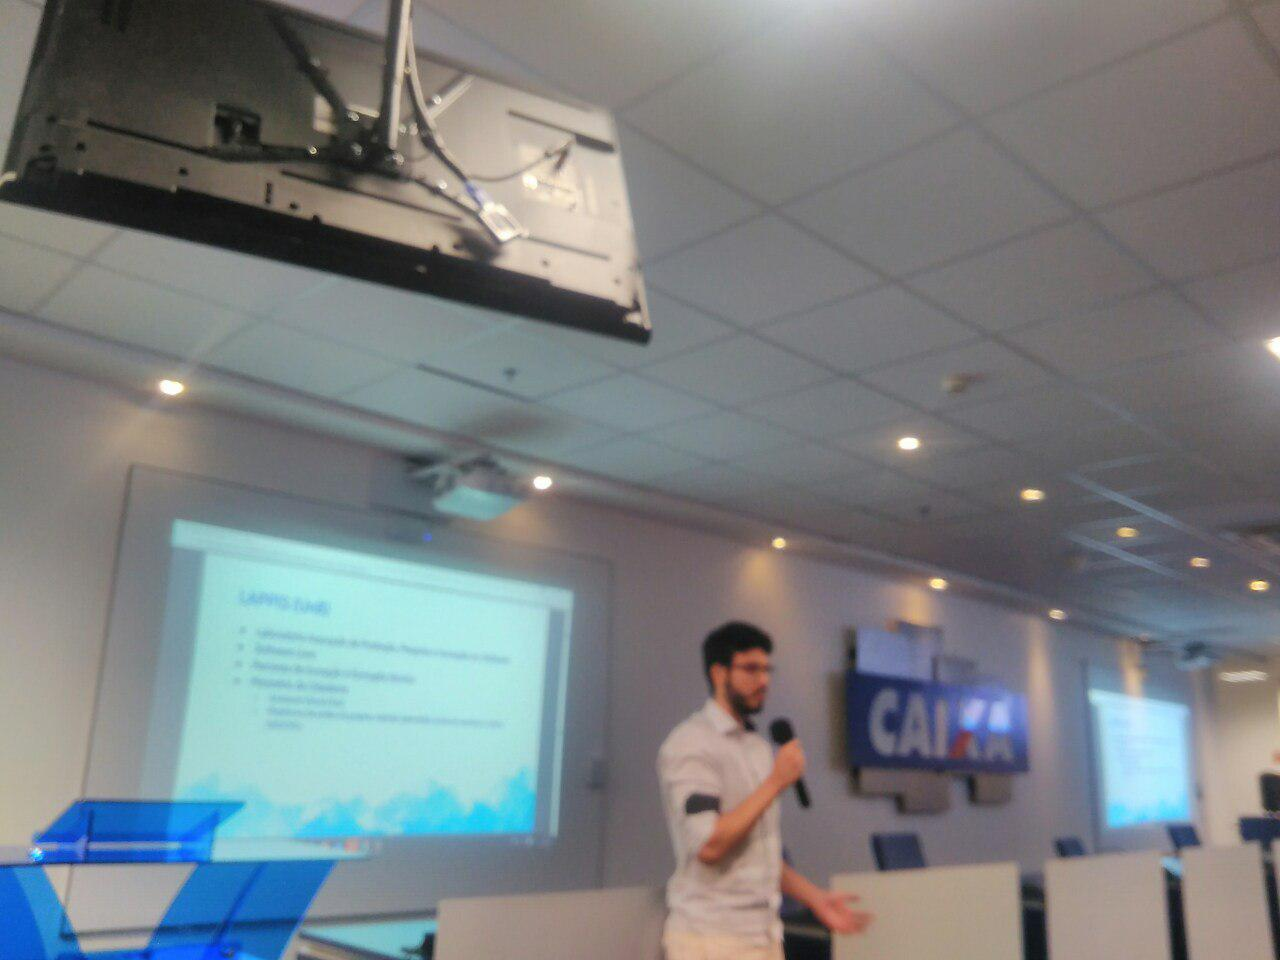
\includegraphics{figs/pydatamoura.jpg}
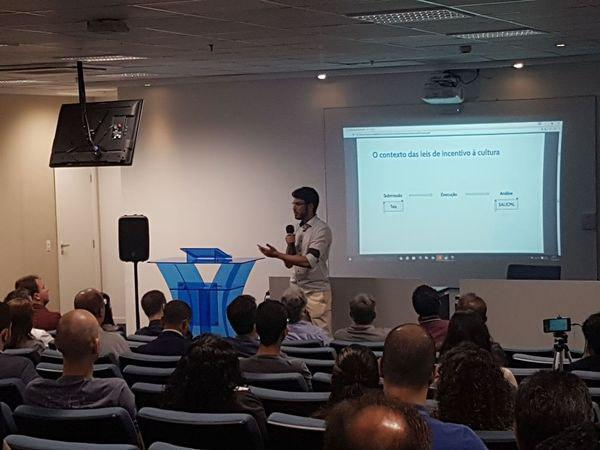
\includegraphics{figs/pydatamoura2.jpg}

\hypertarget{metas-especuxedficas}{%
\subsubsection{Metas Específicas}\label{metas-especuxedficas}}

Quanto as metas específicas dessa frente de trabalho definidas plano de
trabalho são:

\begin{enumerate}
\def\labelenumi{\arabic{enumi}.}
\tightlist
\item
  \textbf{Estudos e documentação do processo de conteinerização, testes
  automatizados, refatoração de sistemas legados em uma estrutura de
  DevOps para viabilizar trabalhos futuros}
\end{enumerate}

\textbf{Concluído}. No início do projeto, fizemos um checklist com as
principais boas práticas, documentações, automações de comunidades de
software livre. Esse checklist foi aplicado em uma lista de projetos
evoluidos e mantidos pelo Ministério da Cultura. Para cada projeto,
colocamos a solução em containers, documentamos o básico (README),
instrumentamos com serviços de análise estática de qualidade de código,
e integração contínua. A importância desse trabalho é que, além de fazer
com que os projetos mantidos pelo ministério façam adesão as práticas
modernas de engenharia de software, permite que outras equipes de
desenvolvimento possam executar, testar e evoluir os projetos mais
facilmente. Adicionalmente, tais ferramentas aceleram a curva de
aprendizado de novos membros no time, além de incentivar boas práticas
de desenvolvimento por meio de monitoramento das métricas.

Essa estratégia, chamada \emph{legacy in the box}, é sugerida na
literatura do estado da prática como primeira ação a ser feita em
direção ao DevOps em sistemas legados. Conteinerizar e instrumentar um
software legado permite que esse seja configurado em um pipeline de
deploy contínuo. A falta de testes cria a vulnerabilidade de se colocar
em ambiente de produção/homologação features defeituosos. Porém esse
risco está presente naturalmente em softwares legados sem testes. Logo,
a estrégia \emph{legacy in the box} agiliza a entrega de novas features,
possibilitando entrega contínua, criação de comunidade, e incentivo as
boas práticas de engenharia de software.

\textbf{Documentação comprobatória}

A lista de projetos que foram refatorado utilizando a estratégia
\emph{legacy in the box} está disponibilizado no
\href{https://github.com/lappis-unb/EcossistemasSWLivre/blob/master/Relatorios/R1/RELATÓRIO\%20ETAPA\%201.pdf}{Relatório
Etapa 1}. O principal benefício dessa estratégia é visto no projeto do
\href{https://github.com/culturagovbr/salic-minc}{Salic}, o principal
software desenvolvido e mantido pelo ministério. Com a estratégia
\emph{legacy in the box} foi possível realizar pipeline de
deploy/entrega contínua e agilizar o processo de deploy. A figura abaixo
mostra o histórico de releases do salic. Pode-se notar que o processo de
release, e logo de deploy/entrega contínua foi adotada somente após a
aplicação da técnica \emph{legacy in the box}. Na imagem, nota-se que
tal técnica possibilitou a realização de até 24 realises em um mês.

\begin{figure}
\centering
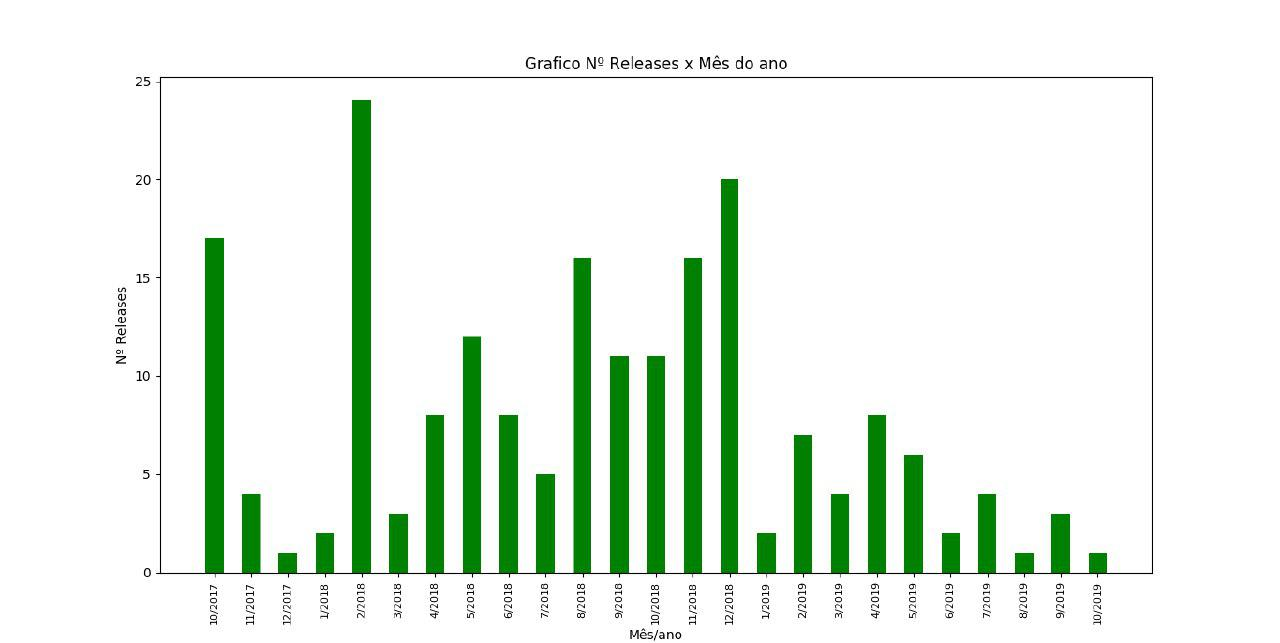
\includegraphics{figs/salic-devops.jpg}
\caption{Fig DevopsSalic}
\end{figure}

\begin{enumerate}
\def\labelenumi{\arabic{enumi}.}
\setcounter{enumi}{1}
\tightlist
\item
  \textbf{Pesquisa em metodologias de refatoração de sistemas legados}
\end{enumerate}

\textbf{Concluído}. O principal problema tratado foi a pesquisa de
estratégias de fazer inovação em plataformas compostas por software
legado. Utilizamos o SALIC, principal software mantido pelo antigo
Ministério da Cultura, que além de ser o maior software ainda é o
software que executa a Lei de Incentivo a Cultura. Nesse contexto,
refatorar e/ou reescrever o Salic é uma tarefa inviável com custos
proibitivos. Uma particularidade do Salic é a quantidade de bancos de
dados (cerca de 10 bancos), e o fato de que várias regras de negócios
estão do próprio banco. A documentação técnica no início do projeto era
mínima, quase inexistente.

Dado o contexto, além da estratégia \emph{legacy in the box}, descrita
na seção acima, pesquisamos e aplicamos outras duas técnicas de
refatoração de sistemas legados. Identificamos o \emph{SalicAPI},
projeto que disponibiliza os dados sobre a execução de projetos da Lei
de incentivo, como sendo o software com o maior pontencial de se ter
comunidade, uma vez que os dados acessados via o \emph{SalicAPI} são de
interesse tanto da sociedade civil quanto de jornalistas. Para o o
\emph{SalicAPI} aplicamos a técnica tradicional de refatoração
orientados a métricas. Para isso, atualizamos a versão do \emph{Python},
automatizamos a execução de testes automatizados, dockerizamos, fizemos
toda a documentação técnica e dos \emph{endpoints}. Essa técnica de
refatoração (reescrita de código, melhoria das práticas, execução de
testes unitários) modernizou o \emph{SalicAPI} e permitiu um pipeline de
entrega/deploy continuo seguro.

A terceira técnica de refatoração de sistemas legados foi no contexto de
inserir novas \emph{features}. Mais especificamente, novas
\emph{features} com inovação em funcionalidades que fazem o
processamento de dados com algoritmos de \emph{machine learning}. Como o
código do SALIC é PHP, e maioria dos frameworks e bibliotecas de
aprendizagem de máquina são desenvolvidos na linguagem \emph{python}.
Por isso, escolhemos a técnica de adotar uma arquitetura microsserviços,
no qual novas funcionalidade são adicionadas a plataforma como novos
microsserviços que compartilham o banco de dados com o software legado.
Essa técnica foi colocada em prática com o serviço \emph{``SalicML''}.
Nele, construimos uma API no qual adicionamos várias métricas de
complexidade de análise de projetos culturais.

\textbf{Documentação comprobatória}

Quanto a estratégia refatoração, foi aplicado ao
\href{https://github.com/lappis-unb/salic-api}{SALIC API}. A figura
abaixo mostra a evolução das métricas relacionadas ao código.

\begin{figure}
\centering
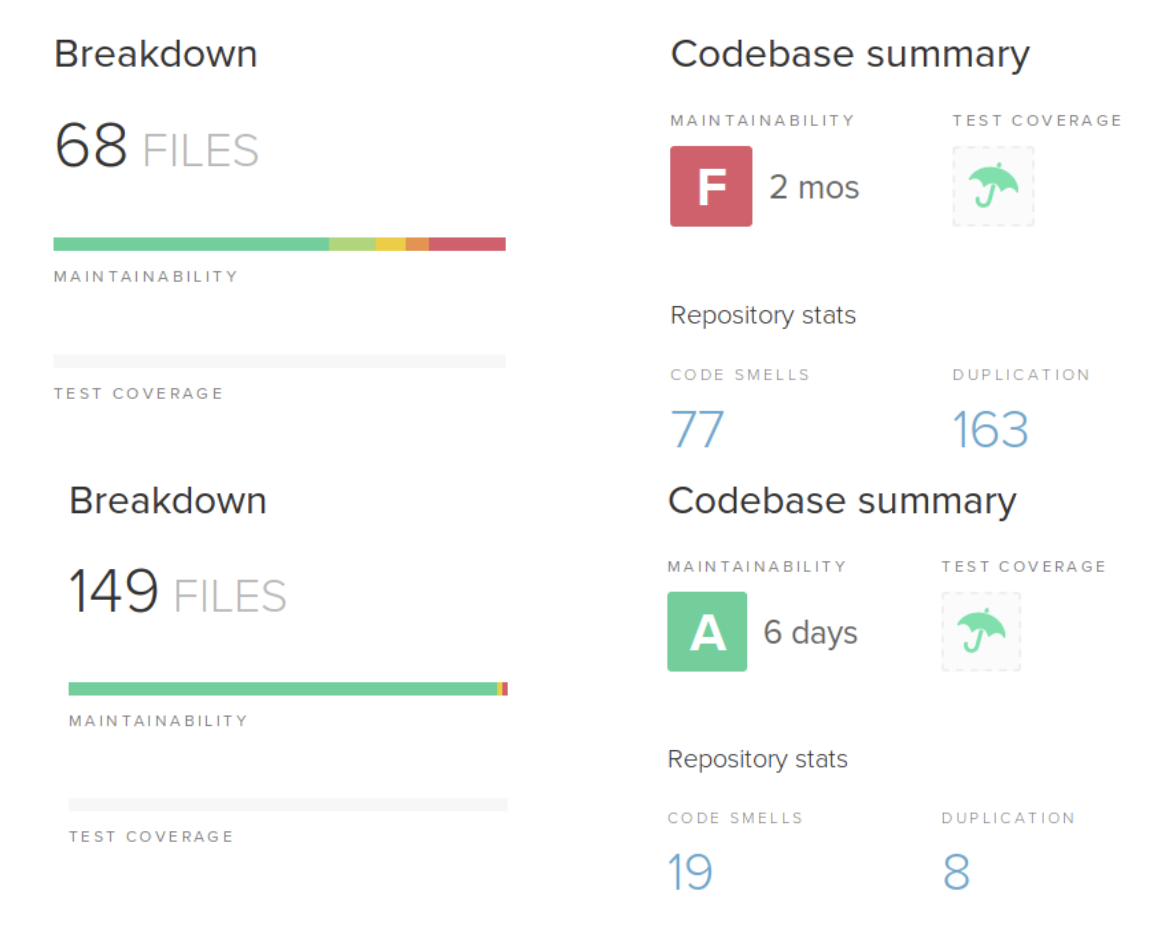
\includegraphics{figs/SALICAPI.png}
\caption{Fig DevopsSalic}
\end{figure}

Além de instrumentar a API com automações como conteiner, integração
contínua (testes automatizados, build, teste de folha de estilo), foi
realizados testes (cobertura atual de 87\%). Foi adicionada também o
graphQL para facilitar a consulta na API. Três docker composers foram
implementados com o ambiente de desenvolvimento, ambiente de homologação
e ambiente de produção. Foi também feito a documentação técnica para
agilizar a manutenção e evolução da API utilizando \emph{readthedocs},
disponibilizado no gitpage
\url{https://salic-api.readthedocs.io/pt/latest/index.html}. Com essa
estratégia, temos o projeto SALIC-API respeitando todas as recomendações
de comunidades \emph{open source}. Com isso, esse projeto, dentre os
mantidos pelo ministério com licenças abertas, é o mais receptivo para
contribuições externas, da comunidade de software.

\begin{figure}
\centering
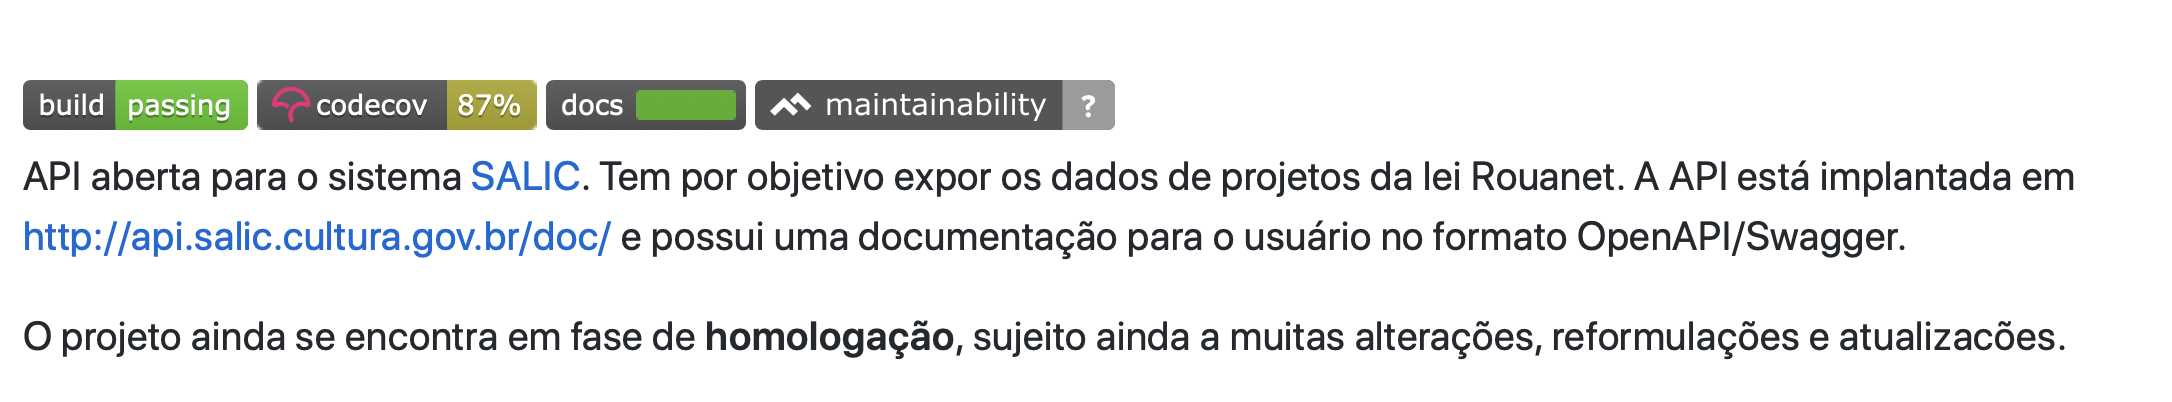
\includegraphics{figs/salicapi2.png}
\caption{Fig DevopsSalic}
\end{figure}

\begin{figure}
\centering
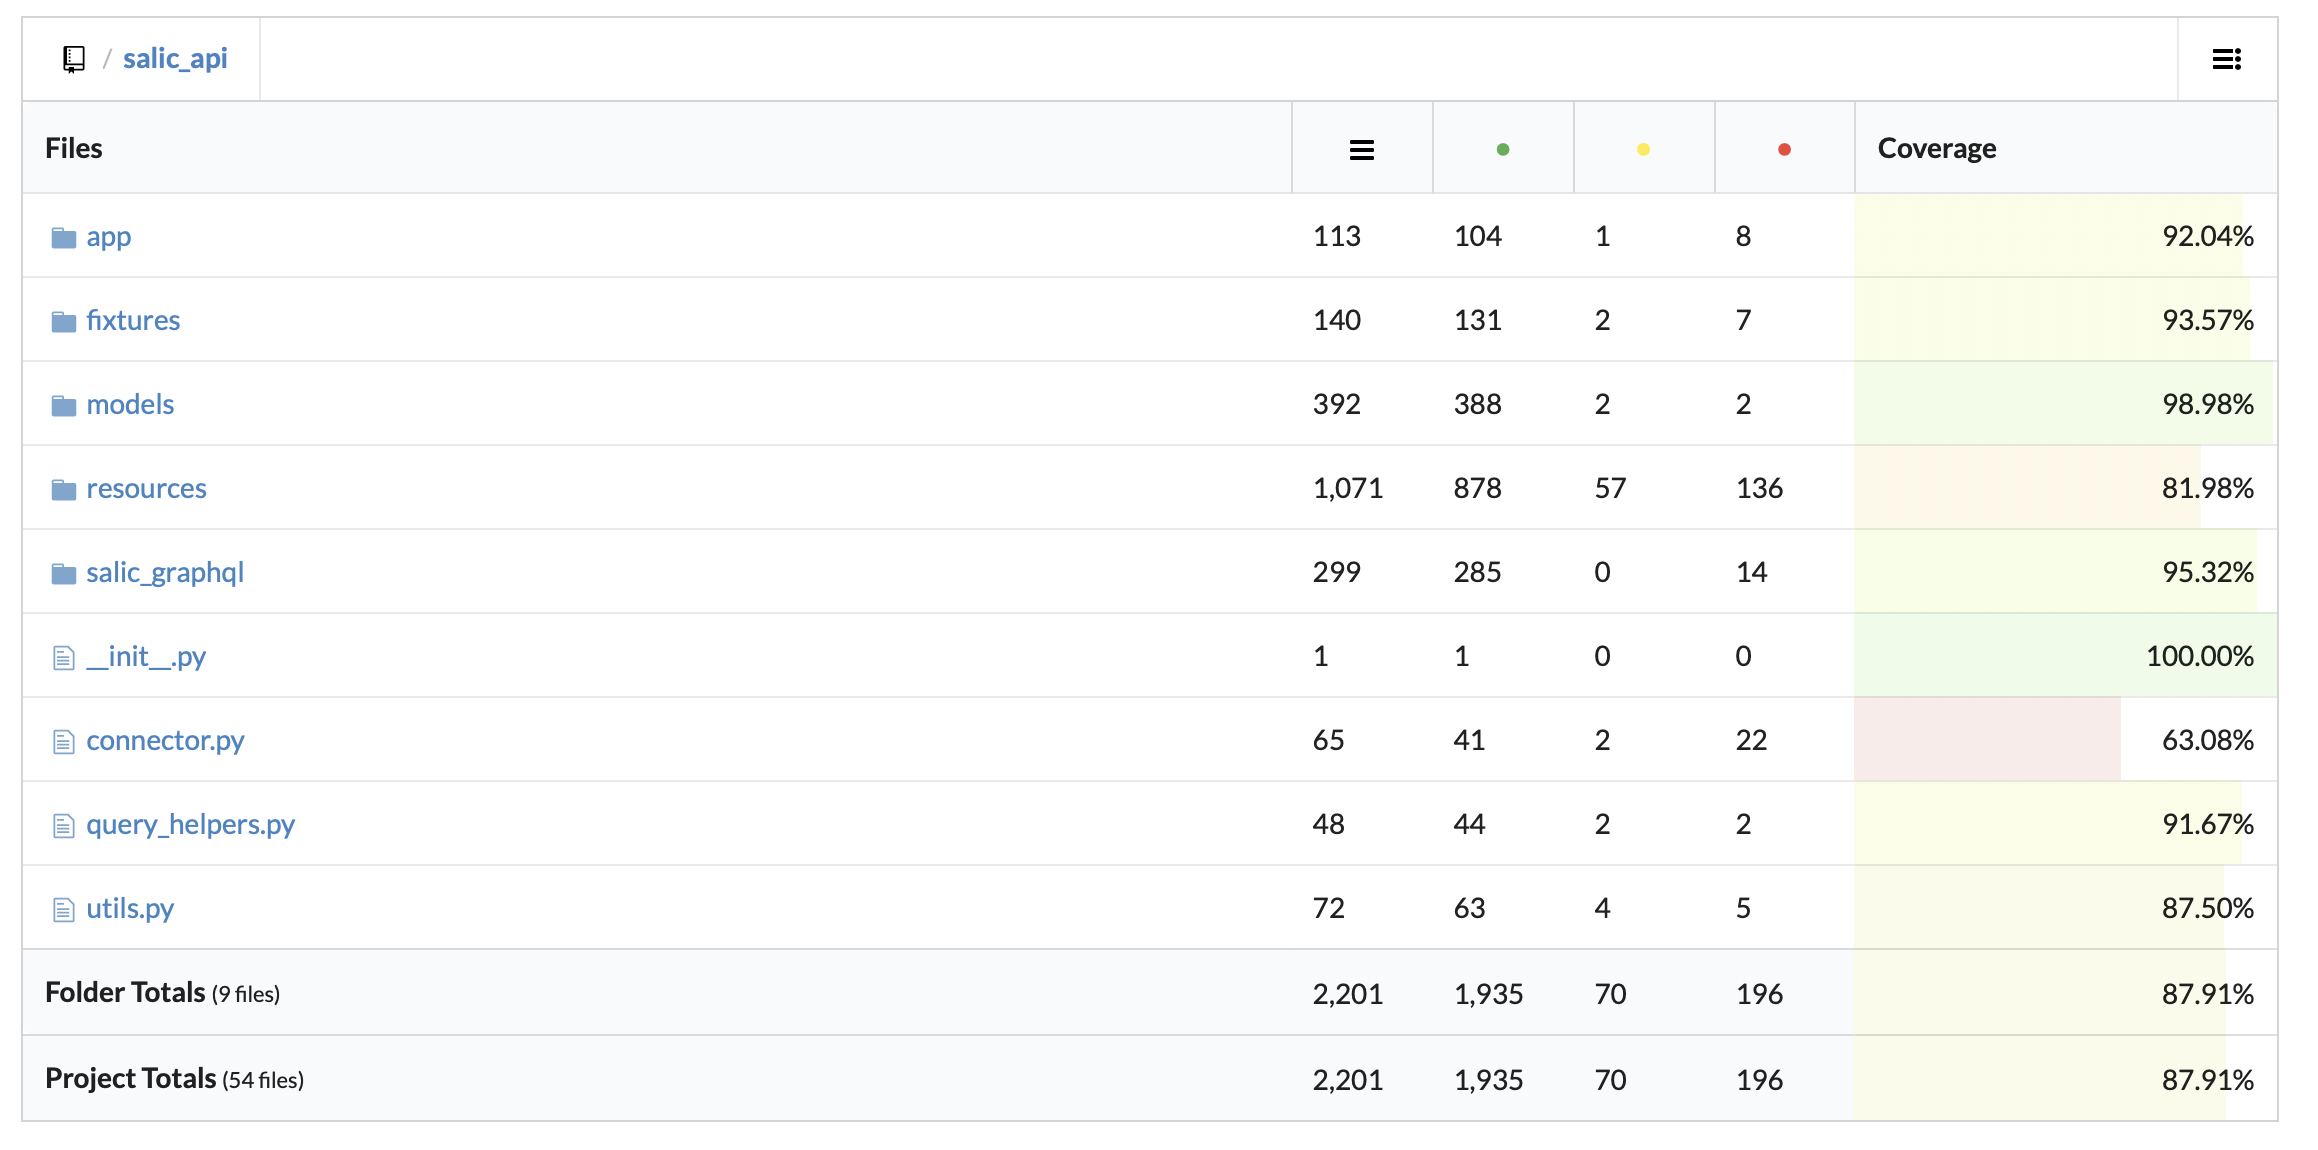
\includegraphics{figs/salicapi1.png}
\caption{Fig DevopsSalic}
\end{figure}

Finalmente, a estratégia de arquitetura microsserviços foi aplicado em
no \href{https://github.com/lappis-unb/salic-ml}{SalicML}.

\begin{enumerate}
\def\labelenumi{\arabic{enumi}.}
\setcounter{enumi}{2}
\tightlist
\item
  \textbf{Utilizar como estudo de casos alguns sistemas legados do
  Ministério da Cultura, tais como o projeto SIMEC (Sistema Integrado de
  Monitoramento Execução e Controle) e o projeto Salic (Sistema de Apoio
  as Leis de Incentivo à Cultura), Sistel}
\end{enumerate}

\textbf{Concluído.}

Dos três projetos citados, trabalhamos com o \emph{SALIC} e o
\emph{Sistel}. No \emph{Sistel} aplicamos a técnica de \emph{legacy in a
box}. Já no \emph{SALIC}, aplicamos as três técnicas pesquisadas:
\emph{legacy in a box}, \emph{refatoração de código orientado a
métricas} e \emph{arquitetura microsserviços}. Toda a documentação
técnica, assim como os resultados técnicos obtidos, e decisões
colaborativas com o Ministério estão disponibilizadas na wiki do
respectivo repositório. Vamos detalhar aqui o trabalho arquitetural
utilizado na estratégia \emph{arquitetura microsserviços}.

Implementar sistemas com modelos de aprendizado de máquina é sempre um
desafio, o trabalho com os dados é o coração da aplicação e deve ter
cuidados especiais. Cada situação tem suas peculiaridades e, no projeto
Salic-ML, não foi diferente. Com o escopo definido ao redor do mundo da
lei de Incentivo a Cultura, o Salic-ML tem como objetivo agilizar
processos pelos quais um projeto cultural deveria passar caso se
candidatasse ao incentivo fiscal.

O uso de aprendizado de máquina e técnicas estatísticas nos dados
disponibilizadas pelo Ministério da Cidadania permitia calcular métricas
que serviam como indicadores de possíveis anormalidades de um projeto,
aumentando a rapidez na busca de eventuais anomalias. A partir desta
situação, surgiu o projeto Salic-ML, nosso objeto de estudo. O objetivo
seria criar uma plataforma na qual, a partir da análise dos dados e por
meio de métricas de cada projeto cultural, indicasse, aos usuários, um
\emph{score} que indicava o quão complexo seria a análise do ponto de
vista financeiro.

O projeto completo está sendo desenvolvido como software livre, e pode
ser acessado em \href{https://github.com/lappis-unb/salic-ml}{SalicML}.

\textbf{Documentação comprobatória}

Grande parte do tempo de projeto foi dedicado aos estudos sobre os dados
disponíveis. Entretanto, toda a análise tinha, como objetivo final, um
produto que pudesse auxiliar os técnicos do Ministério a realizarem o
seu trabalho de uma forma mais otimizada. Para isso, iniciou-se o
trabalho da equipe de produto.

Por conta do tempo e do escopo definido, a arquitetura inicial envolvia
apenas uma aplicação, com fundação no framework web Python Django. A
chamamos de salic-ml-web. Nela, seria possível navegar entre os diversos
projetos disponíveis na base de dados e visualizar uma nota global de
cada um deles, calculada a partir dos algoritmos implementados pela
equipe de data science.

Para viabilizar este comportamento, era necessário integrar os
algoritmos dos Python Notebooks na aplicação Python Django. A solução
encontrada foi transformar o código dos estudos em um pacote Python,
disponibilizado no PyPi e consumido no salic-ml-web.

A divisão da equipe em duas frentes (``Equipe ML'' e ``Equipe ML
Produto'') foi inspirada na abordagem de divisão de serviços por
subdomínio (bem utilizada em arquiteturas de microserviços). O pacote
Python continha os algoritmos resultantes dos estudos sobre os dados e a
aplicação Django tinha maior preocupação em como estes algoritmos seriam
entregues como produto ao Ministério.

Como resultado desta divisão interna, foi planejado o seguinte fluxo de
trabalho:

\begin{enumerate}
\def\labelenumi{\arabic{enumi}.}
\tightlist
\item
  ``Equipe ML'' implementava, no salic-ml, o código do algoritmo
  necessário para calcular uma determinada métrica.
\item
  ``Equipe ML Produto'' preocupava-se em:
\item
  Atualizar, no salic-ml-web, a versão utilizada do salic-ml para
  permitir o uso da nova feature implementada.
\item
  Mostrar os resultados da métrica em um front-end acessível pelos
  técnicos do MinC.
\end{enumerate}

\begin{figure}
\centering
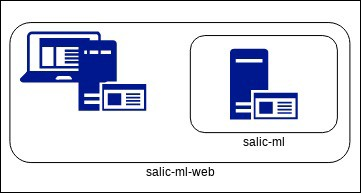
\includegraphics{figs/salicml1.jpg}
\caption{Salicml1}
\end{figure}

As vantagens deste modelo foram:

\begin{itemize}
\tightlist
\item
  Haviam duas equipes e criou-se dois ``serviços''. Cada equipe ficou
  responsável por uma base de código.
\item
  Não observou-se mudanças drásticas das responsabilidades de cada
  equipe, já que o time de ciência de dados permaneceu preocupado em
  criar novos algoritmos e a equipe de produto preocupava-se com outros
  aspectos (DevOps, frontend,~\ldots{}).
\end{itemize}

Entretanto, haviam desvantagens:

\begin{itemize}
\tightlist
\item
  O processo era cascateado: antes, a equipe de data science deveria
  implementar o algoritmo no salic-ml para uso posterior no
  salic-ml-web.
\item
  A separação das equipes gera, naturalmente, eventuais falhas de
  comunicação. Alterações de última hora eram feitas de forma constante
  e isto gerava desgaste dos membros.
\end{itemize}

Para tentar amenizar estes problemas, técnicas de DevOps foram
utilizadas para otimizar o tempo de desenvolvimento de ambos os
projetos. Integração e deploy contínuos permitiam encontrar problemas
mais cedo e, consequentemente, corrigí-los o quanto antes.

Além dos pontos mencionados, havia uma preocupação em relação à
integração com o SALIC, já implementado no Ministério. Para isso, em um
determinado momento, trocou-se o conceito e a arquitetura interna do
salic-ml-web para que ele se tornasse uma API baseada no Django Rest
Framework e que o frontend fosse apenas um protótipo de homologação das
informações, feito em VueJS (salic-ml-frontend). Esperava-se que, em
algum momento, as informações resultantes dos algoritmos fossem
repassadas para o SALIC e que o frontend fosse, no máximo, reutilizado
na integração.

\begin{figure}
\centering
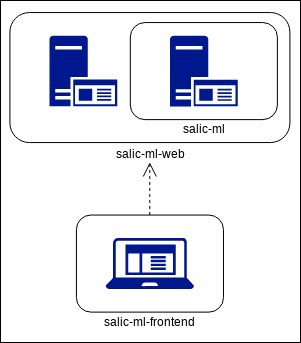
\includegraphics{figs/salicml2.jpg}
\caption{arquitetura após primeira modificação, com frontend separado e
o pacote acoplado no salic-ml-web}
\end{figure}

Dada a implementação do pacote salic-ml, que espelhava o que foi feito
nos Python Notebooks, era necessário alimentar os algoritmos com os
mesmos tipos de input utilizados na fase de data science. Para isso, foi
necessário mapear um Docker Volume, por meio do Docker Compose, para a
pasta na qual o pacote era instalado dentro do contâiner. Nesta pasta,
seriam inseridos os arquivos (.csv) contendo os dados exigidos pelos
algoritmos.

\begin{figure}
\centering
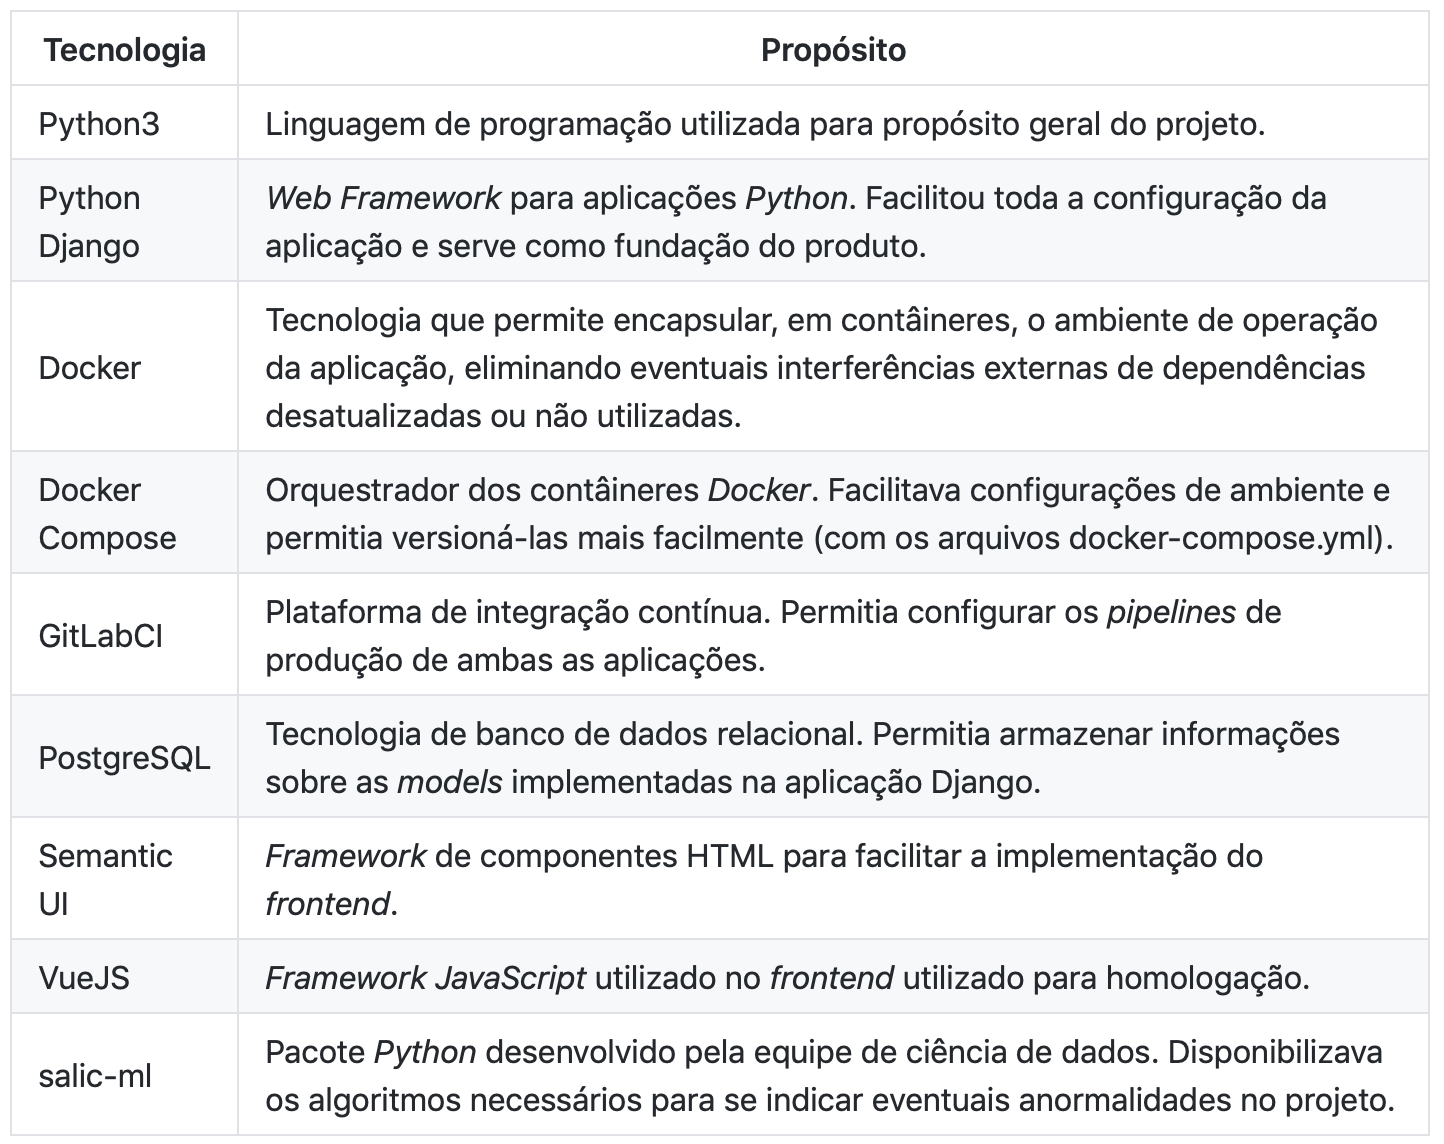
\includegraphics{figs/salicml3.png}
\caption{tecnologias envolvidas na aplicação salic-ml-web}
\end{figure}

Observou-se os seguintes problemas:

\begin{itemize}
\tightlist
\item
  Os~.csv's eram significativamente grandes. Movimentá-los exigia um
  certo tempo e nem sempre era garantido que funcionariam na primeira
  tentativa.
\item
  Instanciar o objeto que continha os algoritmos custava alguns minutos,
  o que causava dificuldades no processo de desenvolvimento do produto.
  Cada modificação mínima no frontend resultava no recarregamento da
  aplicação e, consequentemente, na instanciação deste objeto.
\end{itemize}

Para tentar amenizar o segundo problema, além de serializar o objeto em
um Pickle File, houve uma mudança arquitetural que removeria a
necessidade do salic-ml-web instanciar o objeto que calculava os
algoritmos. Mantendo a ideia do serviço único por equipe, criou-se o
lappis-learning, uma aplicação Python Flask que implementava os
algoritmos resultantes da análise dos dados e disponibilizava os
resultados, em formato de JSON, por meio de uma API. Desta maneira, o
objeto que leva mais tempo para ser instanciado fica completamente
desacoplado da aplicação que exige uma maior cadência de modificações,
facilitando o desenvolvimento.

\begin{figure}
\centering
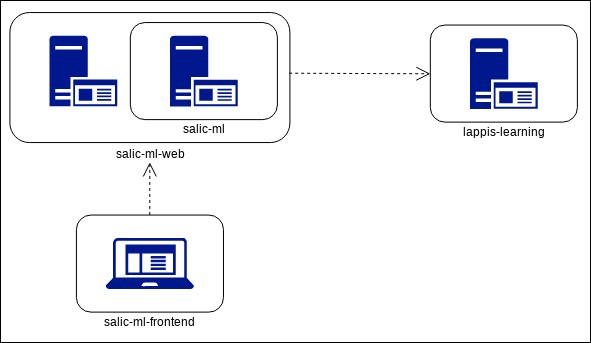
\includegraphics{figs/salicml4.jpg}
\caption{arquitetura resultante após a criação do lappis-learning}
\end{figure}

Aproveitando a modificação arquitetural, optou-se por eliminar o uso
dos~.csv's. A aplicação lappis-learning obtém os dados diretamente do
banco de dados, eliminando a necessidade de se manter os arquivos que os
continham.

Como o estágio de implementação do pacote salic-ml era avançado, a
estratégia de transição envolvia implementar os novos algoritmos
diretamente na nova arquitetura e, aos poucos, iríamos transferindo os
já existentes.

Assim, era possível manter uma arquitetura híbrida. Alguns resultados
eram obtidos do pacote salic-ml, que retornava Python Dicts, e outros do
serviço lappis-learning, que retornava JSONs.

Como pontos de melhoria, é possível observar:

\begin{itemize}
\tightlist
\item
  É um verdadeiro malabarismo técnico manter a arquitetura híbrida do
  ponto de vista de fonte de dados. O cenário ideal seria a finalização
  da transição do consumo do salic-ml para o consumo exclusivo do
  lappis-learning.
\item
  Mesmo com a separação do serviço exclusivo de análise de dados, a
  arquitetura interna deveria possibilitar um cache dos metadados que
  são calculados toda vez que se inicia o serviço lappis-learning.
\item
  A integração, até o momento no qual este texto está sendo escrito, não
  foi realizada.
\end{itemize}

Apesar das possíveis melhorias, também percebemos acertos:

\begin{itemize}
\tightlist
\item
  A separação dos serviços entre as equipes, que beneficiou o
  desenvolvimento como um todo. Haver responsabilidades exclusivas de
  cada equipe possibilitou que cada uma delas pudesse estar mais imersa
  em seus desafios e, consequentemente, apresentar melhores resultados.
\item
  As otimizações internas, como o uso do pickle para agilizar a
  instanciação do objeto que continha os algoritmos.
\item
  A transferência de conhecimento entre os membros foi constante. Seja
  sobre o contexto das leis de incentivo a cultura ou sobre questões
  técnicas, percebe-se que os membros da equipe (tanto do ML quanto do
  ML Produto) tiveram crescimento no conhecimento obtido, o que é
  relevante dado o contexto acadêmico no qual o projeto se inseria.
\end{itemize}

Do ponto de vista arquitetural, apresentamos uma solução que viabiliza o
uso de algoritmos, tanto estatísticos quanto de machine learning, em uma
aplicação web. Já do ponto de vista de produto, conseguimos construir
uma plataforma na qual é possível enxergar anomalias em propostas de
projetos submetidas ao Ministério. O resultado, dentro do escopo e do
contexto presentes na época, foi relevante e apresentou-se de forma
madura aos clientes.

\hypertarget{pacote-de-trabalho-estudo-sobre-catuxe1logos-de-software-culturais}{%
\subsection{Pacote de Trabalho: Estudo sobre catálogos de Software
Culturais}\label{pacote-de-trabalho-estudo-sobre-catuxe1logos-de-software-culturais}}

De acordo com o plano de trabalho, "O foco dessa etapa é executar o
ciclo de projeto de software completo, desde a iniciação. Assim, o
projeto já será iniciado como software livre e com as práticas de
DevOps, ferramentas e tecnologias modernas. Será focado o levantamento
das tecnologias e ferramentas usadas pela comunidade de software livre
para automatizar o processo de desenvolvimento e implantação do
software, pois há pouca pesquisa focada nesse tema. O principal objetivo
nessa etapa é exercitar em todo ciclo de projeto a experimentação e
inovação contínua, de forma a subsidiar a pesquisa realizada na Etapa 5.

Referente à meta ``Realizar estudos sobre funcionalidades de catálogo de
software'' e implemetação de um catálogo de software, foi feito um
levantamento, juntamente com a CGTEC, da necessidade de se desenvolver
um catálogo de software como previsto no plano de trabalho. Foram
levantados como alguns governos lidam com o portifólio de projetos
software livre, tais como as iniciativas do governo inglês de trabalhar
majoritamente com software livre
\url{https://governmenttechnology.blog.gov.uk/2016/12/15/next-steps-for-open-source-in-government/},
e manter seu catálogo de software na própria organização github
\url{http://gds-operations.github.io/}. Observamos também uma tendência
mundial do uso de software livre no governo (egovernment -
\url{http://www.egov4dev.org/success/definitions.shtml}), com uma
quantidade crescente de adesão
\url{https://government.github.com/community/},
\url{https://github.com/g0v}. Observamos que o próprio repositório,
organização, gitpages e wiki do repositório são utilizados para compor o
catálogo de software. Como o principal objetivo dessa etapa é executar
um ciclo completo de projeto, de comum acordo com a CGTEC, decidimos não
desenvolver o catálogo de software, como previsto no calendário. Tal
decisão está documentada e aprovada pelo Ministério no
\href{https://github.com/lappis-unb/EcossistemasSWLivre/blob/master/Relatorios/R3/RELATÓRIO\%20ETAPA\%203.md}{Relatório
de entrega da Etapa 3}.

Vamos detalhar as demais tarefas realizas nesse pacote de trabalho. As
entregas parciais estão disponíveis nos seguintes relatório de entrega
aprovadas pelo ministério:

\begin{itemize}
\item
  \href{https://github.com/lappis-unb/EcossistemasSWLivre/blob/master/Relatorios/R1/RELATÓRIO\%20ETAPA\%201.pdf}{Relatório
  Etapa 1}
\item
  \href{https://github.com/lappis-unb/EcossistemasSWLivre/blob/master/Relatorios/R2/RELATÓRIO\%20ETAPA\%202.pdf}{Relatório
  Etapa 2}
\item
  \href{https://github.com/lappis-unb/EcossistemasSWLivre/blob/master/Relatorios/R3/RELATÓRIO\%20ETAPA\%203.md}{Relatório
  Etapa 3}
\item
  \href{https://github.com/lappis-unb/EcossistemasSWLivre/blob/master/Relatorios/R4/RELATÓRIO\%20ETAPA\%204.pdf}{Relatório
  Etapa 4}
\item
  \href{https://github.com/lappis-unb/EcossistemasSWLivre/blob/master/Relatorios/R5/RELATÓRIO\%20ETAPA\%205.pdf}{Relatório
  Etapa 5}
\item
  \href{https://github.com/lappis-unb/EcossistemasSWLivre/blob/master/Relatorios/R6/RELATÓRIO\%20ETAPA\%206.pdf}{Relatório
  Etapa 6}
\item
  \href{https://github.com/lappis-unb/EcossistemasSWLivre/blob/master/Relatorios/R7/RELATÓRIO\%20ETAPA\%207.pdf}{Relatório
  Etapa 7}
\end{itemize}

\hypertarget{metas-especuxedficas-1}{%
\subsubsection{Metas Específicas}\label{metas-especuxedficas-1}}

\begin{enumerate}
\def\labelenumi{\arabic{enumi}.}
\tightlist
\item
  \textbf{Aplicação de práticas de experimentação e inovação contínua no
  desenvolvimento do projeto de Catálogo de Software Culturais}
\end{enumerate}

\textbf{Cancelado.} Durante a execução do projeto, percebemos que os
objetivos desse pacote de trabalho estavam sendo realizados no
desenvolvimento da TAIS e do SalicML. Adicionalmente, catálogo de
softwares são apresentados atualmente como gitpages dentro das próprias
organizações, otimizando a manutenção e evolução. Dessa forma, em
conjunto acordo com o Ministério, essa frente foi extinta. Tal decisão
foi documentada no relatório de entrega 2 (2 de maio de 2018), página
04, que foi devidamente aprovada pela equipe da gestão do projeto tanto
na Unb quanto no Ministério.

\begin{enumerate}
\def\labelenumi{\arabic{enumi}.}
\setcounter{enumi}{1}
\tightlist
\item
  \textbf{Realizar estudos e documentação do processo de desenvolvimento
  e das boas práticas e automações realizadas}
\end{enumerate}

\textbf{Concluído.} Quanto em relação as boas práticas de documentação
técnica, além de encontros técnicos para apresentação das práticas
experimentadas no laboratório, alguns documentos técnicos foram
elaborados para tal fim. Grande parte do time ficou focado em amadurecer
o pipeline devops, atualizar o pipeline dos softwares do Ministério
trabalhados no laboratório (Salic API, Salic, Mapas culturais), além de
gerar a documentação técnica do conhecimento adquirido. Experimentamos
várias formas de documentação técnica foram realizados durante o
projeto. No projeto Tais, experimentamos realizar documentos técnicos de
estudos precedentes a tomada de decisão. Tais estudos foram todos
disponibilizados na wiki do projeto. Já o SalicML, experimentados a
documentação técnica dos experimentos de data science disponíveis nos
notebooks, nos quais o código está junto com a documentação técnica. No
SalicAPI, utilizamos documentação técnica \emph{readthedocs} para
registrar tando as funcionalidades implementadas, quanto o roadmap do
projeto. Finalmente, testamos os benefícios na realização de webinários
como forma de documentação e compartilhamento de conhecimento, forma de
treinamento. Todas essas formas de documentação são amplamente
utilizadas pela comunidade opensource, e percebemos que cada contexto
sugere um modelo próprio. A partir da nossa experiência, vimos que o
formato de documentação técnica mais adequada para um projeto opensource
é o formato adotado pela comunidade. Por exemplo, em comunidade de
software livre que tratam de problemas de machine learning, ciência de
dados, e processamento de sinais, o uso de notebooks para documentação
técnica é o padrão adotado.

\textbf{Documentação comprobatória} - Parte da documentação de DevOpsfoi
disponibilizada no repositório do laboratório em
https://gitlab.com/lappis-unb/docs, disponibilizada também como anexo no
final deste documento, os documentos cobrem tanto a primeira quanto a
terceira meta do período.

Foi elaborado documentação/relatório descrevendo todo o pipeline usado
para deploy contínuo no laboratório com os seguintes tutoriais, que
podem ser aplicados em diversos contextos:

\begin{enumerate}
\def\labelenumi{\arabic{enumi}.}
\tightlist
\item
  GitLab CI/CD: Guia relacionado ao uso da Integração Contínua e Deploy
  contínuo no Gitlab;
\item
  Overview e exemplo básico(pt-br): Um guia que ensina como usar o
  gitlab CI/CD para gerar integração contínua e deploy contínuo em um
  projeto básico;
\item
  Usando Docker Compose (pt-br): Um guia que ensina como usar o GitLab
  CI/CD para gerar integração contínua com o Docker Compose em um
  projeto ágil;
\item
  Integrando GitLab CI/CD com projeto GitHub(pt-br): Um procedimento que
  possibilita o uso do GitLab CI/CD no projeto GitHub.
\end{enumerate}

Toda a documentação foi realizada em português e disponibilizada para
acesso.

\begin{itemize}
\tightlist
\item
  Documentação técnica da Tais - Wiki do projeto
  \url{https://github.com/lappis-unb/tais/wiki/}
\item
  Documentação Técnica do SalicML - Notebooks do projeto
  \url{https://github.com/lappis-unb/salic-ml/tree/master/notebooks}
\item
  Documentação técnica do Salic API - readthedocs
  \url{https://salic-api.readthedocs.io/pt/latest/} e swagger
  \url{http://api.salic.cultura.gov.br/doc/}
\item
  Documentação Promova Cultura - wiki do projeto
  \url{https://github.com/lappis-unb/PromovaCultura/wiki}
\end{itemize}

Um exemplo da documentação técnica de estudos da Tais está apresentado
abaixo (os demais estarão disponíveis como anexo e disponíveis no
repositório do projeto):

\hypertarget{estudo-de-muxe9tricas-para-bots}{%
\subsubsection{Estudo de Métricas para
Bots}\label{estudo-de-muxe9tricas-para-bots}}

  Este documento contém um estudo sobre métricas relevantes para o
contexto de um(a) assistente virtual.

  O objetivo deste estudo é encontrar métricas que possam contribuir
para a análise da dados da interação entre o usuário-bot, auxiliando na
área de \emph{business} e de desenvolvimento.

\hypertarget{muxe9tricas}{%
\subsubsection{Métricas}\label{muxe9tricas}}

  Uma métrica é uma medida quantificável que é usada para rastrear e
avaliar o status de um processo específico.

  Os próximos dois subtópicos serão responsáveis por expor as métricas
que foram definidas como apropriadas para a área de negócio e de
desenvolvimento, no contexto da Tais.

\hypertarget{muxe9tricas-de-neguxf3cio}{%
\paragraph{Métricas de Negócio}\label{muxe9tricas-de-neguxf3cio}}

\begin{itemize}
\tightlist
\item
  \textbf{Quantidade de usuários totais}
\end{itemize}

    Medir a quantidade de usuários/sessões que já interagiram com a
Tais. As medidas podem variar de acordo com o intervalo de tempo
definido (por dia, por semana, por mês, \ldots{}).

\begin{itemize}
\tightlist
\item
  \textbf{Interações por usuário {[}IU{]}}
\end{itemize}

    Quantificar a média de perguntas realizadas por usuário.

    IU = (Qtd. total de perguntas do usuário) / (Qtd. total de usuários)

\begin{itemize}
\tightlist
\item
  \textbf{Horas com mais atividades}
\end{itemize}

    Identificar em qual horário os usuários mais interagem com o bot.
Definir por intervalo de tempo (De 11:00 as 12:30, etc).

\begin{itemize}
\tightlist
\item
  \textbf{Perguntas mais frequentes}
\end{itemize}

    Analisar as perguntas que são feitas com mais frequências.

    Neste caso, pode-se definir como a pergunta mais realizada em todo o
tempo, ou então a pergunta que foi tendência em determinado intervalo de
tempo.

\begin{itemize}
\tightlist
\item
  \textbf{Taxa de satisfação}
\end{itemize}

    Medida que diz respeito a taxa de satisfação em relação ao serviço
prestado pelo bot. Se o assistente virtual está conseguindo suprir as
necessidades do usuário e em qual ``qualidade''.

\begin{itemize}
\tightlist
\item
  \textbf{Self-service rate}
\end{itemize}

    Quantos usuários conseguem atingir o seu objetivo com a conversa,
sem a interação externa de um humano.

\begin{itemize}
\tightlist
\item
  \textbf{Retention Rate}
\end{itemize}

    Quantos usuários retornam a interagir com a assistente virtual. Esta
métrica pode se relacionar, também, com o intervalo de tempo entre cada
sessão do usuário.

    É importante identificar também se após retornar o objetivo do
usuário é diferente do anterior. Porque pode sinalizar que suas dúvidas
não foram sanadas anteriormente.

\hypertarget{muxe9tricas-de-desenvolvimento}{%
\paragraph{Métricas de
Desenvolvimento}\label{muxe9tricas-de-desenvolvimento}}

\begin{itemize}
\tightlist
\item
  \textbf{Taxa de confusão (CR)}
\end{itemize}

    Calcular a quantidade de \emph{fallbacks} em relação a quantidade de
perguntas realizadas pelos usuários.

    CR = (Qtd. de \emph{fallbacks}) / (Qtd. total de perguntas)

\begin{itemize}
\tightlist
\item
  \textbf{Frases/palavras mais frequentes}
\end{itemize}

    Analisar as frases/palavras que são mais realizadas. Neste caso,
pode-se definir também como as palavras mais realizadas em todo o tempo,
ou então a que foi tendência em determinado intervalo de tempo.

\begin{itemize}
\tightlist
\item
  \textbf{Perguntas mais frequentes}
\end{itemize}

    Analisar as perguntas que são feitas com mais frequências. Neste
caso, pode-se definir como a pergunta mais realizada em todo o tempo, ou
então a pergunta que foi tendência em determinado intervalo de tempo.

\begin{itemize}
\tightlist
\item
  \textbf{Etapas de conversação}
\end{itemize}

    Calcular a quantidade média de etapas realizadas por sessão. Uma
etapa é definida por uma inteção do usuário e a resposta do bot.

    As conversas que excedem significativamente ou ficam aquém da média
da etapa de conversação geralmente indicam uma experiência ruim para o
usuário.

\begin{itemize}
\tightlist
\item
  \textbf{Fallback por intent}
\end{itemize}

    Identificar quais são as intenções de usuários que mais geram
\emph{fallbacks}.

\begin{itemize}
\tightlist
\item
  \textbf{Fluxo de sessão}
\end{itemize}

    Um fluxograma que mostra o ``caminho'' percorrido pelos usuários em
cada sessão de conversa e a porcentagem de cada ``caminho''.
Relacionando também com a métrica anterior de \textbf{\emph{Fallback}
por intent}, a qual identifica em qual intenção o bot entrou no
fallback.

\hypertarget{links-das-referuxeancias}{%
\subsubsection{Links das referências}\label{links-das-referuxeancias}}

\begin{itemize}
\tightlist
\item
  http://www.topbots.com/5-bot-metrics-every-chatbot-should-track/
\item
  https://blog.ubisend.com/optimise-chatbots/right-chatbot-kpi
\item
  https://blog.growthbot.org/the-practical-guide-to-chatbot-metrics-and-analytics
\item
  https://chatbotsmagazine.com/chatbot-analytics-101-e73ba7013f00
\end{itemize}

\begin{enumerate}
\def\labelenumi{\arabic{enumi}.}
\setcounter{enumi}{2}
\tightlist
\item
  \textbf{Relatório com os modelos de desenvolvimento e comunidade para
  serem aplicados aos projetos de software do Minc}
\end{enumerate}

\textbf{Concluído} - O projeto foi dividido em ciclos de 3 meses, no
qual a cada ciclo era realizado um planejamento estratético com a equipe
estratégica do Ministério da Cidadania (tanto a equipe de coordenação
quanto de negócio). Nessa reunião de planejamento estratégico,
amadurecido ao longo do projeto, era definido as metas estratéficas para
o próximo ciclo, além das épicas priorizadas. Essas reuniões foram
documentadas na wiki do repositório ou em apresentações com o
alinhamento. Então, a equipe se reunia para criar as issues, histórias
de usuário e tarefas a serem desenvolvidas. Tais tarefas estão todas
documentadas em forma de issue, no repositório de cada repositório.
Utilizamos \emph{sprints} de duas semanas para planejar e revisar o
desenvolvimento. A cada mês, a equipe técnica/gestão da TI do ministério
era convidado para visitar o laboratório e acompanhar a evolução das
frentes.

Em relação as automações realizadas, elas foram tomas mapeadas nas
\emph{issues} e toda documentação técnica necessária para evoluir e
manter as soluções.

Como o desenvolvimento do catálogo de software foi cancelado, tanto as
práticas quanto métodos e automações, além da documentação foi usada nos
outros projetos desenvolvidos, como o projeto da Tais e SalicML.

\textbf{Documentação comprobatória} O processo de construção
colaborativa do planejamento e execução contínua foi feito em
colaboração com o Ministério. Abaixo colocamos um exemplo do resultado
de um planejamento estratégico da Etapa I.

\hypertarget{planejamento-estratuxe9gico-etapa-1---e1}{%
\subsubsection{Planejamento Estratégico Etapa 1 -
E1}\label{planejamento-estratuxe9gico-etapa-1---e1}}

Planejamento referente a Etapa I do projeto (Novembro 2017 a Fevereiro
2018)

\begin{enumerate}
\def\labelenumi{\arabic{enumi}.}
\tightlist
\item
  Levantamento de necessidades Etapa I - Nitai + time Lappis - 07/11
\item
  Proposta Planejamento Estratégico Etapa I- Time Lappis - 14/11
\item
  Aprovação Planejamento Estratégico Etapa I - Time Lappis + Time MinC -
  22/11
\end{enumerate}

\hypertarget{metas-estratuxe9gicas}{%
\paragraph{Metas Estratégicas}\label{metas-estratuxe9gicas}}

\begin{itemize}
\tightlist
\item
  Primeiros passos para transformar software culturais para dinâmica de
  práticas colaborativas e aberta
  (\href{https://github.com/lappis-unb/EcossistemasSWLivre/wiki/Metas\#meta-1-transforma\%C3\%A7\%C3\%A3o-de-software-legado-em-comunidades-de-software-aberto}{meta
  estratégica 1})
\item
  Desburocratizar o acesso a lei Rouanet (proposta)~
\end{itemize}

\hypertarget{uxe9picas}{%
\paragraph{Épicas}\label{uxe9picas}}

\begin{enumerate}
\def\labelenumi{\arabic{enumi}.}
\tightlist
\item
  Avaliar sociabilidade de software culturais ao ecossistema de SWL
\item
  Começar cultura de entrega contínua de SW
\item
  Avaliação do fluxo de preenchimento de proposta
\item
  Escrever documentos de visão de cada frente de trabalho
\end{enumerate}

\hypertarget{features}{%
\paragraph{Features}\label{features}}

\hypertarget{avaliar-sociabilidade-de-software-culturais-ao-ecossistema-de-swl}{%
\subparagraph{1. Avaliar sociabilidade de software culturais ao
ecossistema de
SWL}\label{avaliar-sociabilidade-de-software-culturais-ao-ecossistema-de-swl}}

\begin{itemize}
\tightlist
\item
  {[}x{]} diagnóstico do repositório para a comunidade (mapas)
\item
  {[}x{]} prognóstico do repositório para a comunidade (mapas)
\item
  {[}x{]} diagnóstico do repositório para a comunidade (salic-br)
\item
  {[}x{]} prognóstico do repositório para a comunidade (salic-br)
\end{itemize}

\hypertarget{comeuxe7ar-cultura-de-entrega-contuxednua-de-sw}{%
\subparagraph{2. Começar cultura de entrega contínua de
SW}\label{comeuxe7ar-cultura-de-entrega-contuxednua-de-sw}}

\begin{itemize}
\tightlist
\item
  {[}x{]} Criação de uma stack de desenvolvimento
\item
  {[}x{]} Criação do mecanismo de chatops que auxilie a equipe na gestão
  da infra-estrutura
\item
  {[}x{]} Criação de uma stack de análise Graylog para aferição da saúde
  dos serviços e da infra-estrutura.
\item
  {[}x{]} monitorar/visualizar o fluxo de trabalho da TI do MinC
\end{itemize}

\hypertarget{avaliauxe7uxe3o-do-fluxo-de-preenchimento-de-proposta}{%
\subparagraph{3. Avaliação do fluxo de preenchimento de
proposta}\label{avaliauxe7uxe3o-do-fluxo-de-preenchimento-de-proposta}}

\begin{itemize}
\tightlist
\item
  {[}x{]} Escolha das estratégias e ferramentas de Machine Learning para
  o chatbot
\item
  {[}x{]} Elaboração e implementação da interação inicial do chatbot
  para o portal da Lei Rouanet
\item
  {[}x{]} Treinamento e refinamento das informações e técnicas
  utilizadas no chatbot
\item
  {[}x{]} diagnostico de UX (salic-minc)
\end{itemize}

Os planejamentos estratégicos foram sempre agendados via email e as
decisões registradas nos emails, e registradas em issues/apresentações e
wiki do projeto. Abaixo estão os tipos de emails trocados para esse fim.
Em anexo vamos colocar alguns das apresentações realizadas tanto para o
planejmanento estratégico quanto para oficialização das entregas.

\begin{figure}
\centering
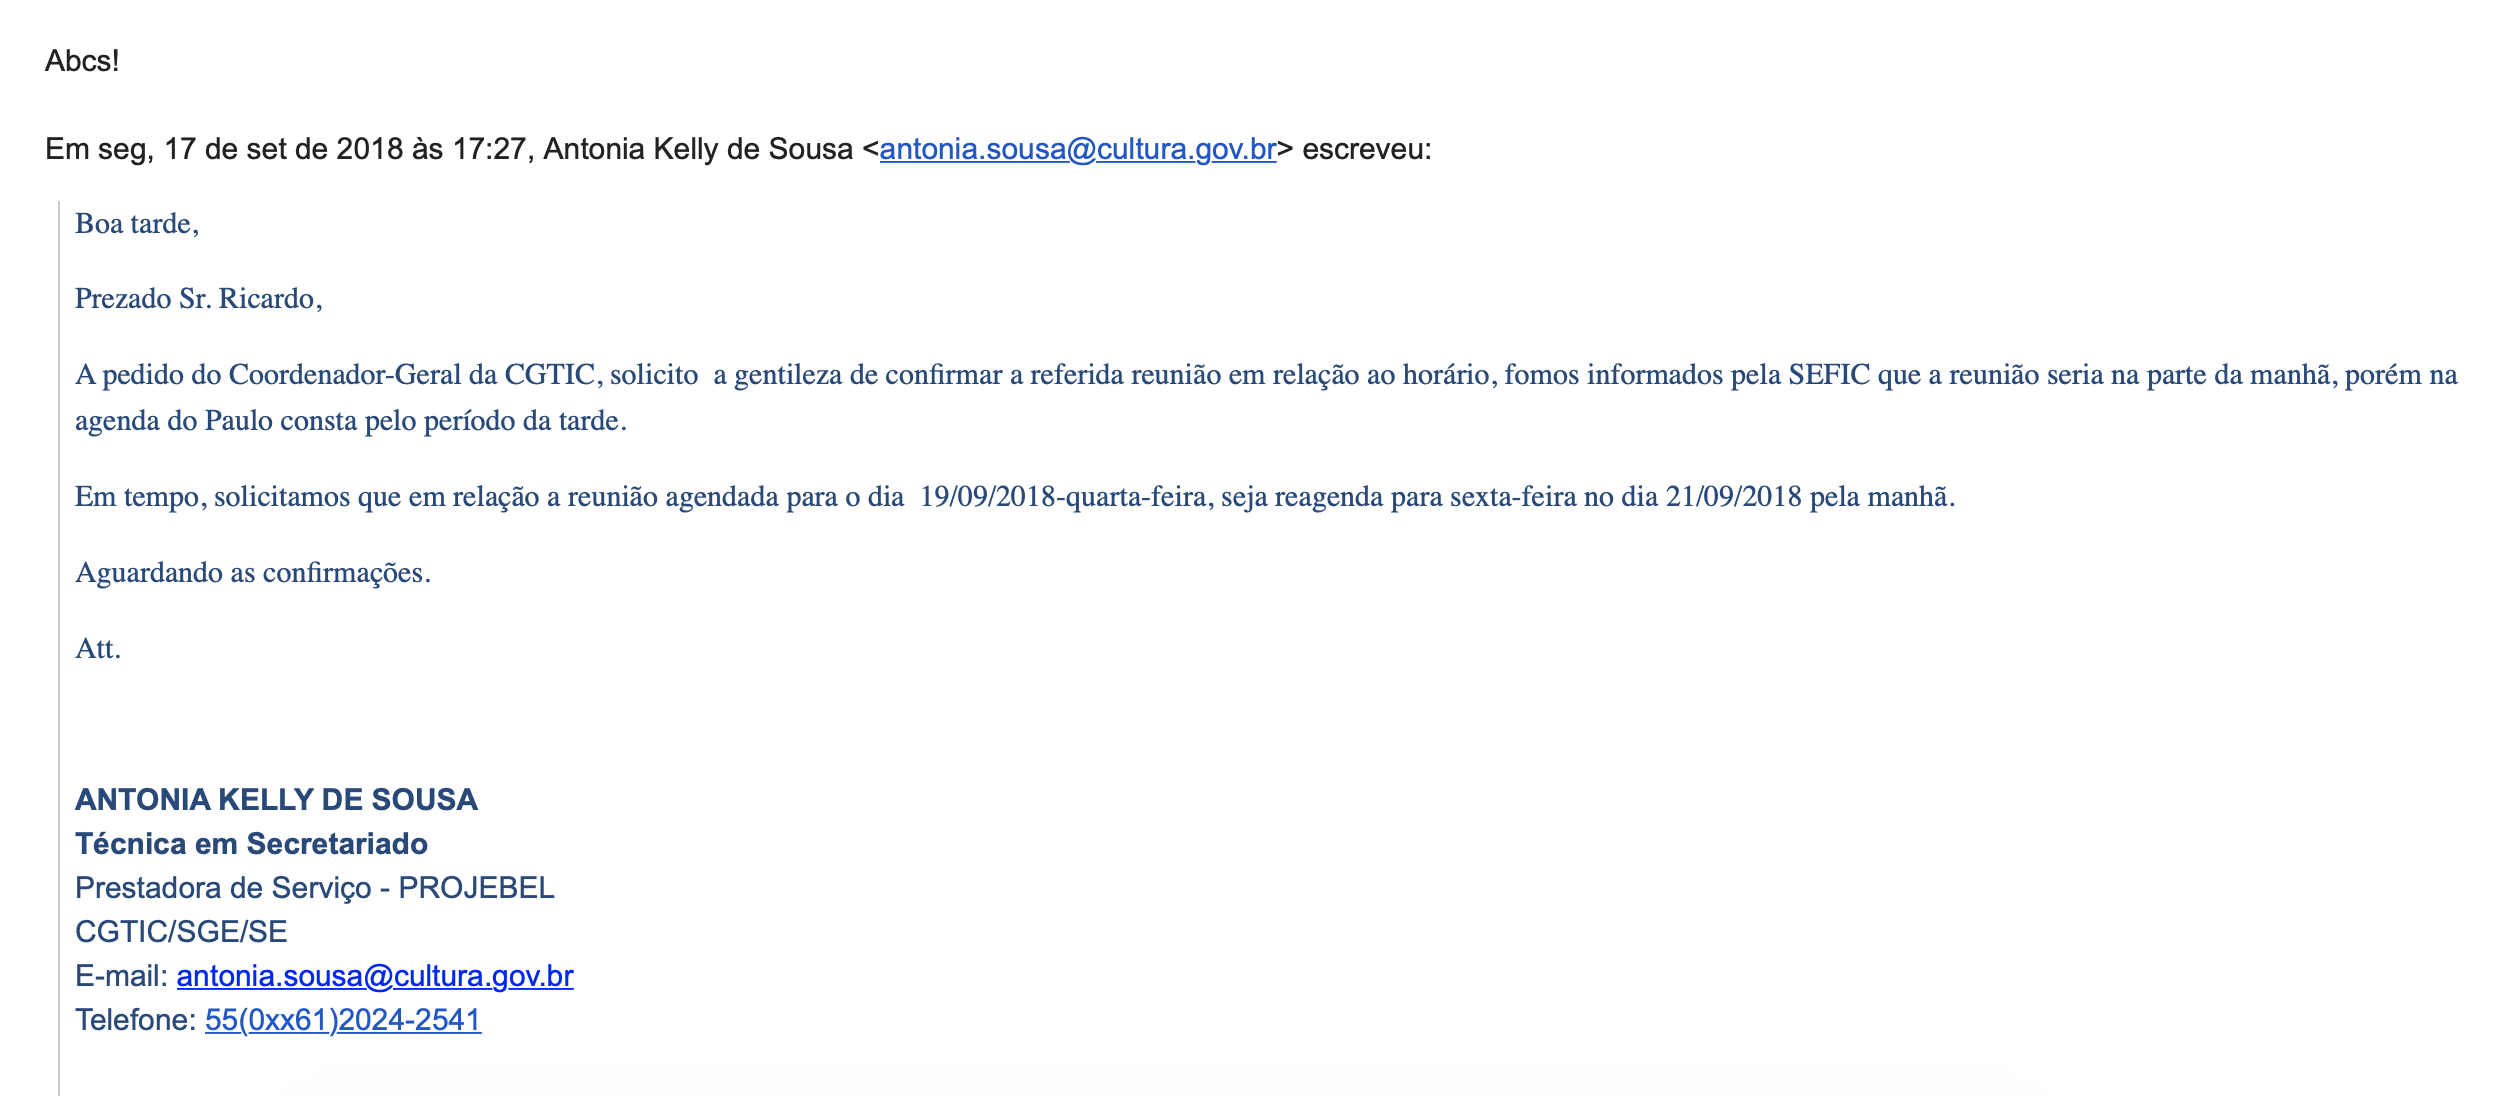
\includegraphics{figs/estrategico.png}
\caption{Reuniao estrategica}
\end{figure}

\begin{figure}
\centering
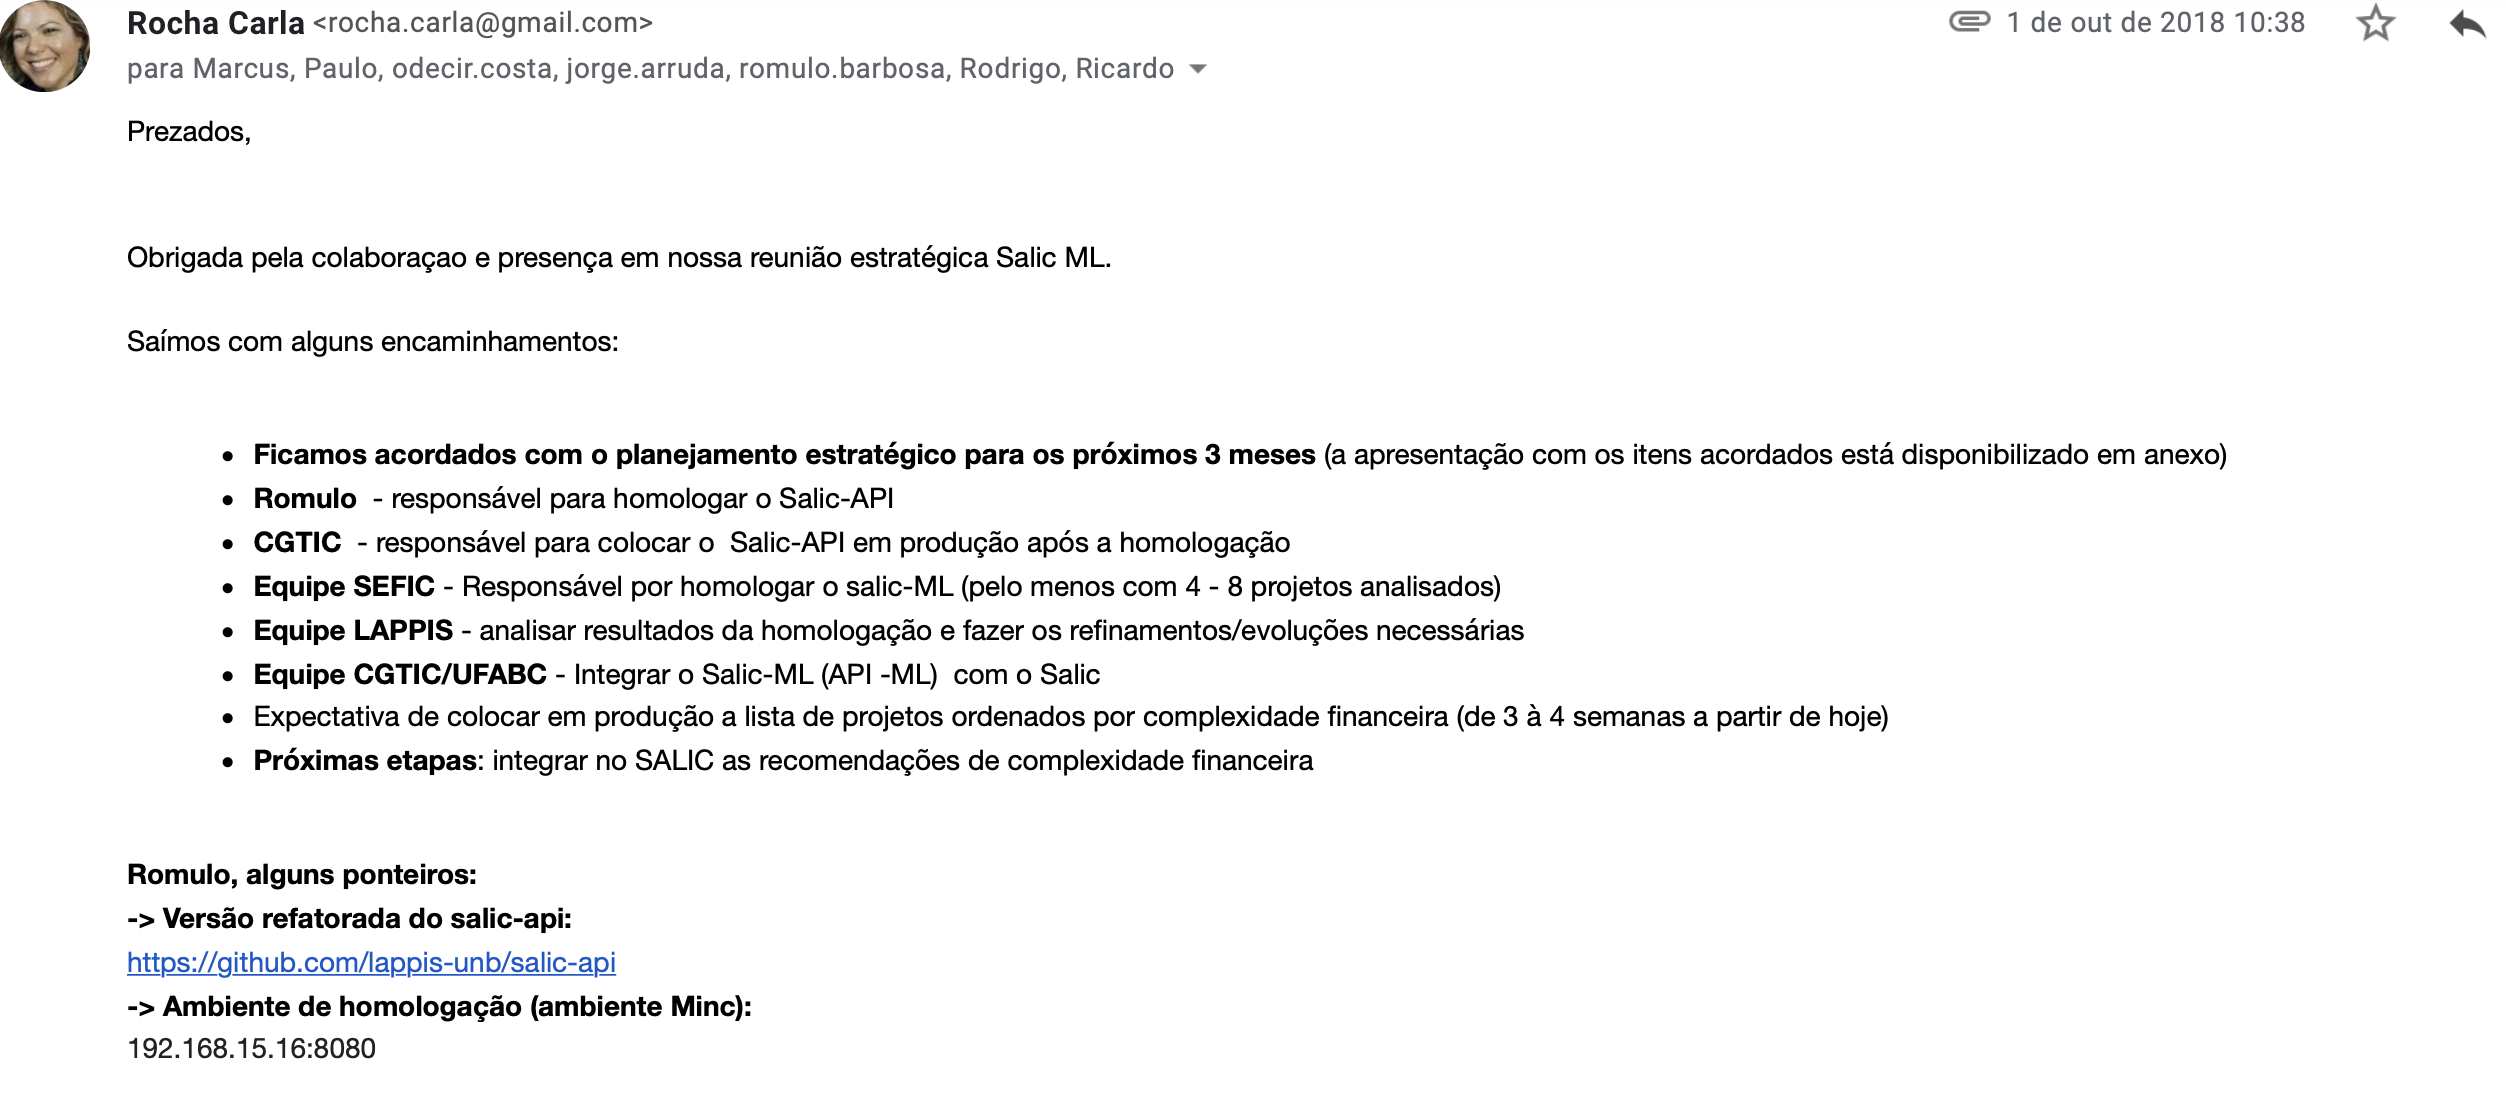
\includegraphics{figs/estrategico1.png}
\caption{Reuniao estrategica 1}
\end{figure}

Além dos relatórios de entregas trimestrais que são aprovadas pelo
Ministério, a documentação completa dos planejamentos estratégicos e
execução desses ciclos estão disponíveis na wiki do projeto
\url{https://github.com/lappis-unb/EcossistemasSWLivre/wiki} e em
apresentações que serão disponibilizada nos anexos. Após o planejamento
estratégico, cada time trabalhou de forma auto organizada para o
planejamento das sprints, priorização das issues, e alocação de
recursos. Para título de exemplo, o projeto Tais tem ao total de 30
sprints (milestones) e um total de 387 issues fechadas. Um resumo de
como os principais repositórios se organizaram em issues está
apresentado na próxima imagem.

\begin{figure}
\centering
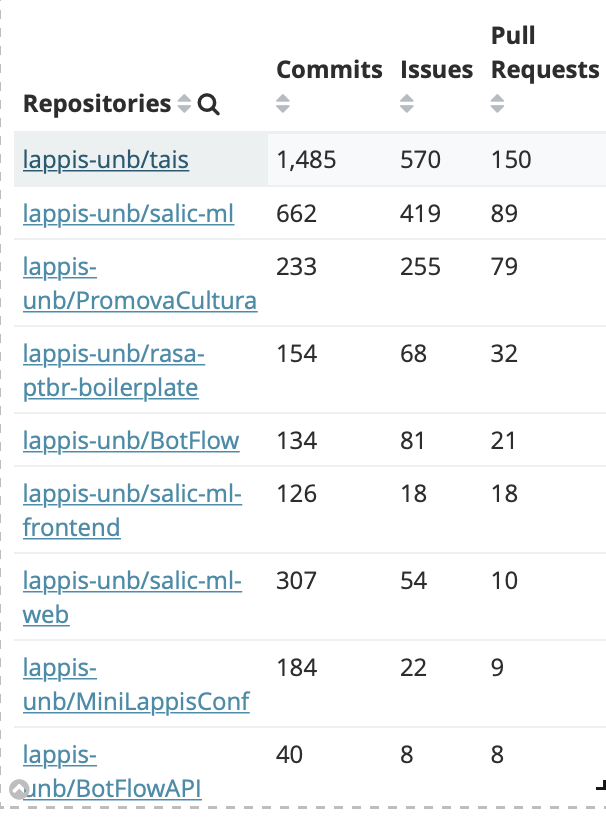
\includegraphics{figs/total.png}
\caption{resumo dos repositorios}
\end{figure}

\begin{enumerate}
\def\labelenumi{\arabic{enumi}.}
\setcounter{enumi}{3}
\tightlist
\item
  \textbf{Transferência de conhecimento e capacitar a equipe de
  servidores e técnicos do MinC em práticas de gestão e desenvolvimento
  de software aberto, colaborativo e contínuo}
\end{enumerate}

\textbf{Concluído} - Durante toda a execução do projeto, tivemos a
preocupação em manter a documentação técnica atualizada para deixar a
comunidade dos projetos desenvolvidas receptivas. Além disso, realizamos
ao longo do projeto diversos workshops de Devops, chatbots, ML, boas
práticas, com a equipe técnica do ministério treinamentos. Ao amadurecer
tecnicamente conhecimento sobre chatbots e a arquitetura da Tais,
realizamos diversos webinares que estão disponibilizados no youtube, que
abordam diversos aspectos técnicos importantes para a manutenção e
evolução da Tais. Participamos também de 2 edições do pydata gravadas no
qual apresentamos a visão geral da Tais e do SalicML. Tais materiais
estão organizados e disponibilizados de forma que pessoas interessadas
em manter e evoluir os projetos desenvolvidos no projeto terão todo o
apoio técnico necessário.

\textbf{Documentação comprobatória} - A transferência e capacitação da
equipe técnica do ministério foi realizada de forma contínua. Diversos
workshops foram realizadas no laboratório. Parte da capacitação é
possível por meio de documentação técnica e webinar, seguindo padrões de
comunidades opensource. Em anexo ao presente relatório serão
apresentados todos os eventos de capacitação realizados ao longo do
projeto.

Alguns exemplos de capacitações realizadas:

\begin{itemize}
\tightlist
\item
  Entrega Técnica Ciclo trimestral (15/08/2018) e workshop devops - A
  equipe Técnica do Ministério reuniu com a equipe projeto Ecossistemas
  para apresentação das entregas realizadas no ciclo trimestral de
  desenvolvimento e um workhop mão na massa devops.
\end{itemize}

\begin{figure}
\centering
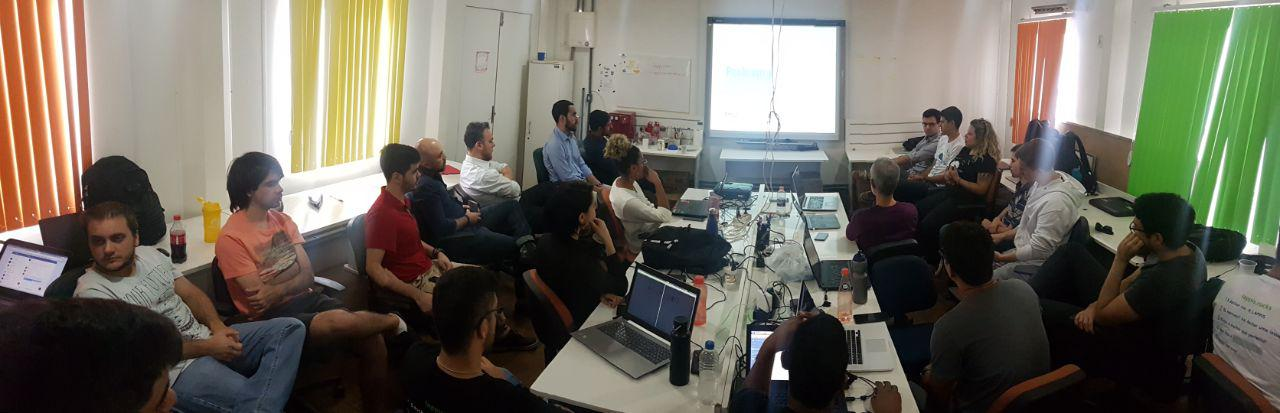
\includegraphics{figs/entrega1.jpg}
\caption{Alt text}
\end{figure}

\begin{itemize}
\tightlist
\item
  LabConf (31/08/2018) - LabConf, ou Conferência dos laboratórios de
  inovação da cultura, foi o evento organizado pelo LAPPIS no Ministério
  da Cultura para que o arranjo de TED entre Universidade e o Ministério
  da Cultura pudesse ser discutido. Nesse dia, os demais laboratório
  (UFG, UFABC, UnB) puderam apresentar os avanços alcançados em seus
  respectivos projetos, diversos workshops práticos relacionados a
  DevOps foram ministrados pelos bolsistas do LAPPIS, e mesas rendondas
  foram realizadas para discutir modelos de contratação.
\end{itemize}

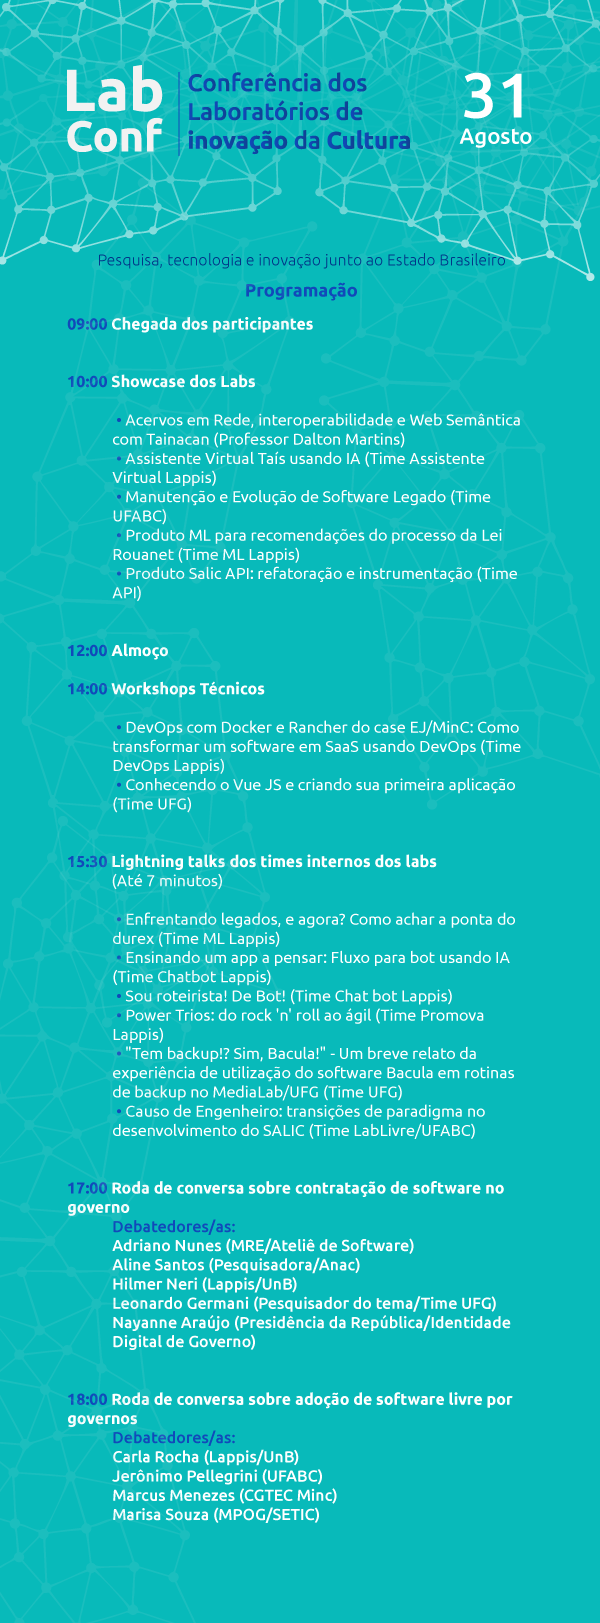
\includegraphics{figs/labconf.png} 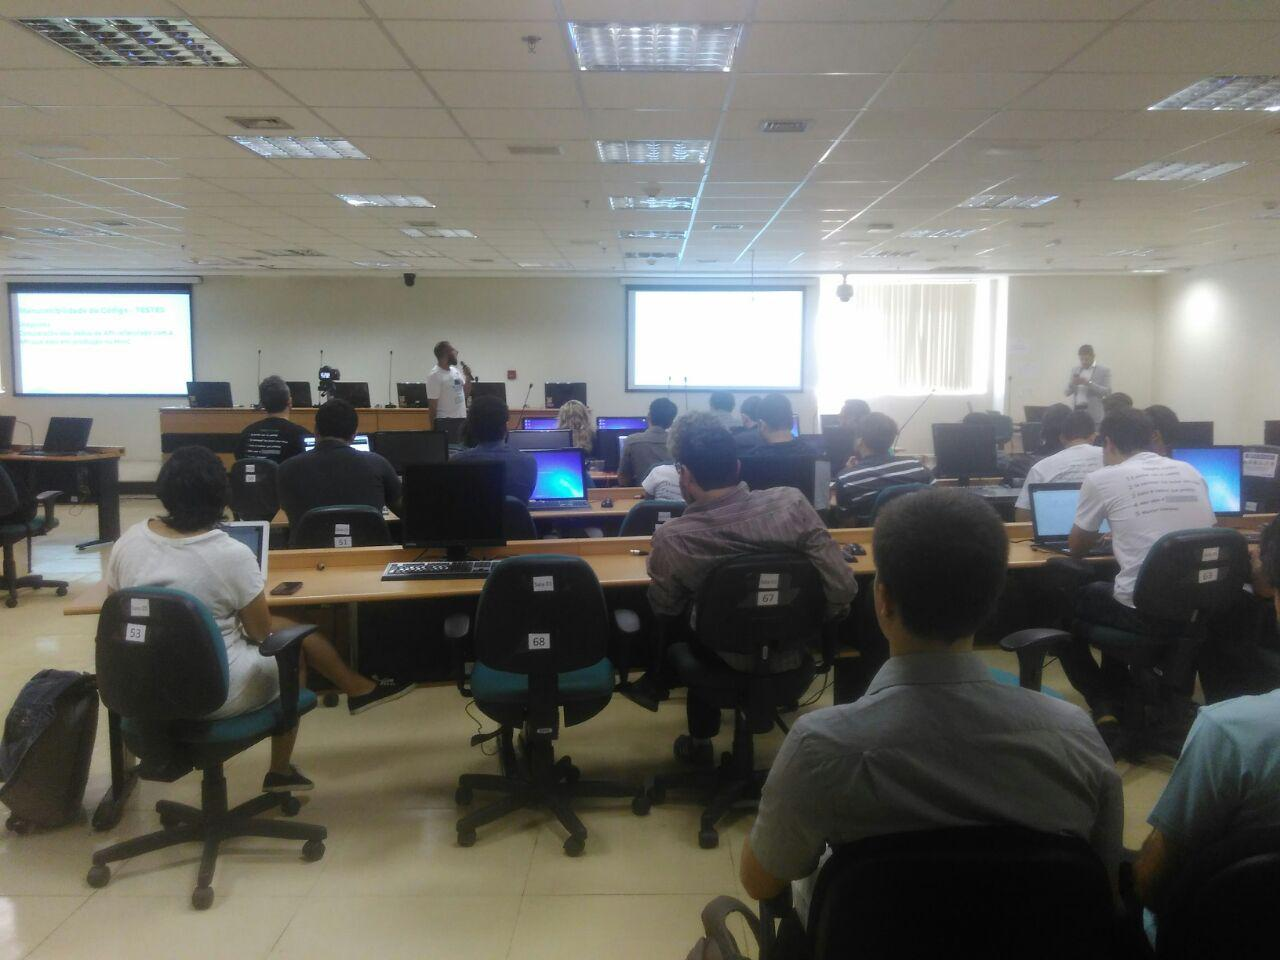
\includegraphics{figs/labconf2.jpg}

\begin{itemize}
\tightlist
\item
  Webinar - Métricas importantes para chatbots - Autor(es): Guilherme
  Lacerda e Bruna Pinos
  \url{https://www.youtube.com/watch?v=yqzxZsOa3gg}
\end{itemize}

\begin{figure}
\centering
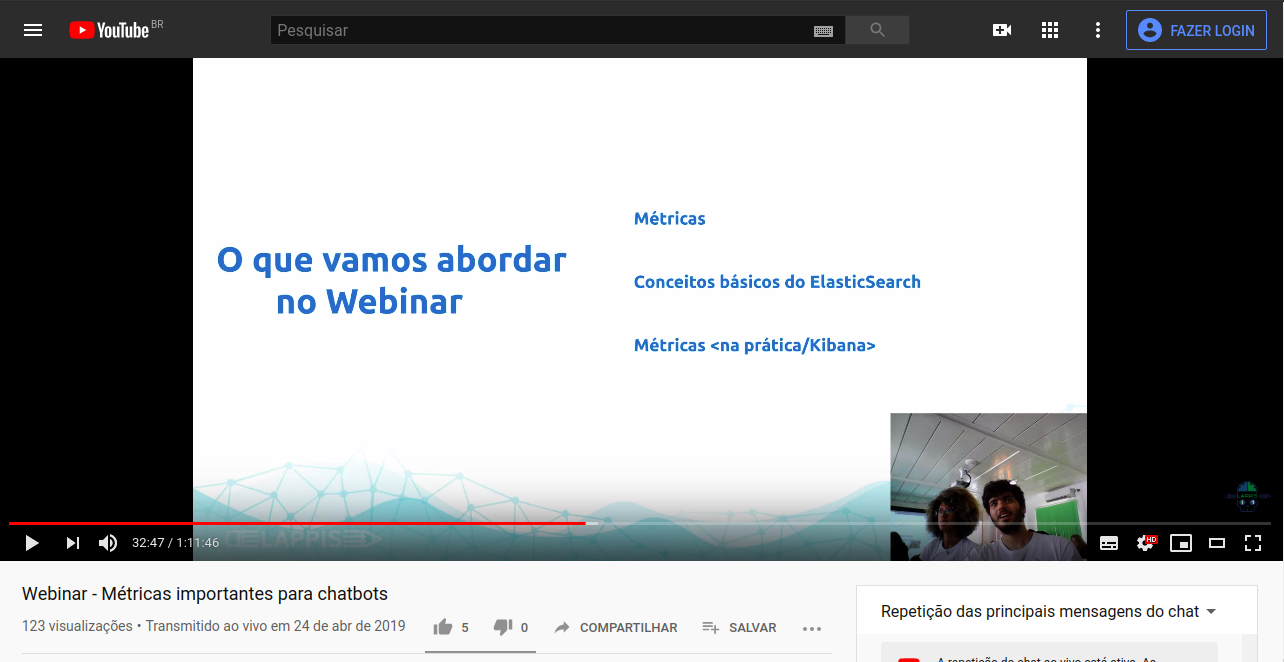
\includegraphics{figs/webinar_metricas_importantes.png}
\caption{Webinar metricas}
\end{figure}

\begin{figure}
\centering
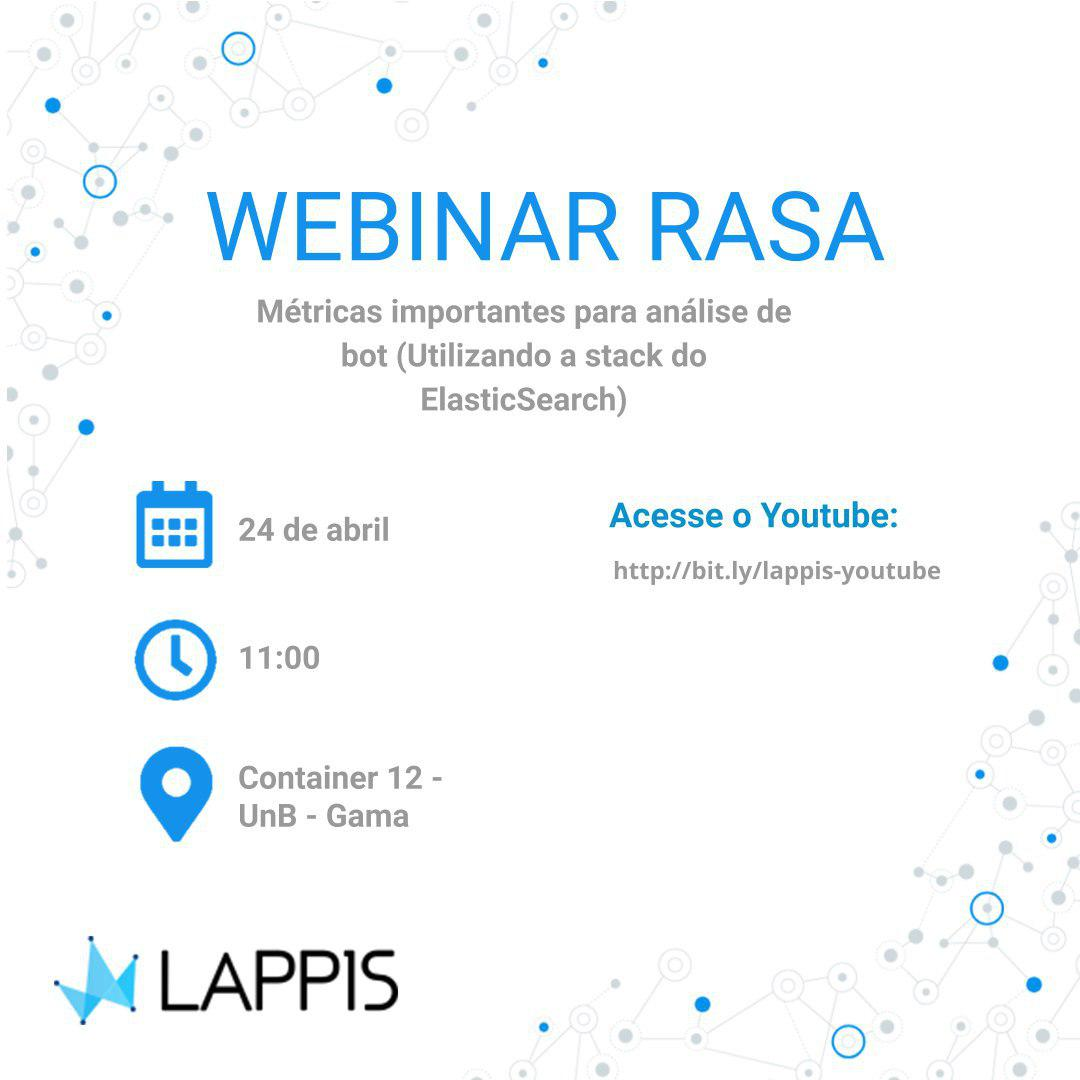
\includegraphics{figs/webinar24-04.jpg}
\caption{Alt text}
\end{figure}

A lista completa de atividades de capacitação realizadas ao longo do
projeto estão em anexo. Algumas dessas iniciativas/eventos foram
aprovados nos relatórios de entregas parciais:

\begin{itemize}
\item
  Relatório Etapa 2 -
  \url{https://github.com/lappis-unb/EcossistemasSWLivre/blob/master/Relatorios/R2/RELATÓRIO\%20ETAPA\%202.pdf}
\item
  Relatório Etapa 5 -
  \url{https://github.com/lappis-unb/EcossistemasSWLivre/blob/master/Relatorios/R5/RELATÓRIO\%20ETAPA\%205.pdf}
\item
  Relatório Etapa 6 -
  \url{https://github.com/lappis-unb/EcossistemasSWLivre/blob/master/Relatorios/R6/RELATÓRIO\%20ETAPA\%206.pdf}
\item
  Relatório Etapa 7 -
  \url{https://github.com/lappis-unb/EcossistemasSWLivre/blob/master/Relatorios/R7/RELATÓRIO\%20ETAPA\%207.pdf}
\end{itemize}

\hypertarget{pacote-de-trabalho-estudos-sobre-pruxe1ticas-de-gestuxe3o-colaborativa-em-comunidades-de-software-aberto}{%
\subsection{Pacote de Trabalho: Estudos sobre práticas de gestão
colaborativa em comunidades de software
aberto}\label{pacote-de-trabalho-estudos-sobre-pruxe1ticas-de-gestuxe3o-colaborativa-em-comunidades-de-software-aberto}}

De acordo com o plano de trabalho, ``O principal resultado dessa
pesquisa será sistematizar e produzir conhecimento sobre as práticas das
comunidades de software livre que o Estado participa por adesão e, a
partir dos aprendizados com seus arranjos, orientar e capacitar os
servidores e técnicos do MinC nas práticas de planejamento, gestão de
softwares abertos, aprimorando os mecanismos de governança digital dos
softwares presentes no portifólio do MinC''.

\hypertarget{metas-especuxedficas-2}{%
\subsubsection{Metas Específicas}\label{metas-especuxedficas-2}}

\begin{enumerate}
\def\labelenumi{\arabic{enumi}.}
\tightlist
\item
  \textbf{Estudos de caso sobre comunidades de software livre onde o
  Estado participa por adesão, com prioridade para os softwares
  utilizados para a gestão cultural}
\end{enumerate}

\textbf{Concluído}

\textbf{Documentação comprobatória} -

\begin{enumerate}
\def\labelenumi{\arabic{enumi}.}
\setcounter{enumi}{1}
\tightlist
\item
  \textbf{Estudos sobre boas práticas para planejamento conjunto de
  milestones e releases entre as organizações que fazem parte das
  comunidades} \textbf{Concluído} -
\end{enumerate}

\textbf{Documentação comprobatória} -

\begin{enumerate}
\def\labelenumi{\arabic{enumi}.}
\setcounter{enumi}{2}
\tightlist
\item
  \textbf{Estudos sobre boas práticas de comunicação e mobilização no
  contexto das comunidades onde o Estado participa}
\end{enumerate}

\textbf{Concluído} -

\textbf{Documentação comprobatória} -

\begin{enumerate}
\def\labelenumi{\arabic{enumi}.}
\setcounter{enumi}{3}
\tightlist
\item
  \textbf{Participação em eventos e encontros das comunidades de
  software livre que contribuem para o portifólio mantido pelo MinC}
\end{enumerate}

\textbf{Concluído} -

\textbf{Documentação comprobatória} -

\begin{enumerate}
\def\labelenumi{\arabic{enumi}.}
\setcounter{enumi}{4}
\tightlist
\item
  \textbf{Estudos sobre arranjos econômicos utilizados pelas comunidades
  com fins de sustentabilidade de seus comuns de software}
\end{enumerate}

\textbf{Concluído} -

\textbf{Documentação comprobatória} -

\begin{enumerate}
\def\labelenumi{\arabic{enumi}.}
\setcounter{enumi}{5}
\tightlist
\item
  \textbf{Estudos sobre metodologias e suportes tecnológicos para a
  gestão colaborativa em comunidades de software livre nas quais o
  Estado participa por adesão}
\end{enumerate}

\textbf{Concluído} -

\textbf{Documentação comprobatória} -

\hypertarget{pacote-de-trabalho-estudo-de-tuxe9cnicas-de-aprendizado-de-muxe1quina-para-apoiar-a-fiscalizauxe7uxe3o-da-lei-rouanet}{%
\subsection{Pacote de Trabalho: Estudo de técnicas de Aprendizado de
Máquina para apoiar a fiscalização da Lei
Rouanet}\label{pacote-de-trabalho-estudo-de-tuxe9cnicas-de-aprendizado-de-muxe1quina-para-apoiar-a-fiscalizauxe7uxe3o-da-lei-rouanet}}

De acordo com o plano de trabalho, ``O principal objetivo é o estudo de
técnicas de Aprendizado de Máquina que possam apoiar o sistema de
recomendação e fiscalização da lei Rouanet. Nessa etapa será realizada
uma pesquisa exploratória em técnicas de aprendizado de máquina e
processamento de linguagem natural. Tais técnicas e algoritmos serão
aplicados para melhorar a experiência de usuário (UX) por meio da
proposta de chatbots como interface entre os proponentes na lei Rouanet
e o Ministério da Cultura''.

\hypertarget{metas-especuxedficas-3}{%
\subsubsection{Metas específicas}\label{metas-especuxedficas-3}}

\begin{enumerate}
\def\labelenumi{\arabic{enumi}.}
\tightlist
\item
  \textbf{Realizar estudos e propor técnicas de processamento de
  linguagem natural, aprendizado supervisionado e o desenvolvimento de
  chatbots para interagir com proponentes da Lei Rouanet}
\end{enumerate}

\textbf{Concluído} - Principal pesquisa do projeto TAIS. Durante o
projeto foram testados diversos frameworks de chatbots, dentre eles o
\emph{hubot natural}, \emph{botpress}, e \emph{rasa}. O objetivo era
pesquisar os algoritmos, dados de treinamento e performance de
algoritmos de processamento de linguagem natural em português. Pela
novidade da tecnologia, e das ferramentas, existia poucos ou nenhum
experimento executado em português.

Após diversos experimentos, testes (a primeira versão da Tais utilizamos
o \emph{hubot natural} com o classificador Support Vector Machine),
escolhemos o Rasa, pois além de crescente comunidade, possuia a vantagem
de trazer a possibilidade de customizar o pipeline de processamento e
algoritmos. Além disso, já estava implementado algoritmos modernos de
processmanto de linguagem natural, tais como \emph{Embeddings},
\emph{LSTM}, entre outros.

Testamos diversas técnicas de classificadores de intenção do usuário:
Support Vector Machine (SVM), Embeddings. Após diversos experimentos
observamos que o embeddings classificava melhor com poucos dados de
treinamento, que é o caso do chatbot em português que tem poucos ddos
para treinamento. Além de testes de algoritmos de \emph{Natural Language
Processing} (NLU), um chatbot tem que prever a ação mais adequadava a
partir da intenção do usuário e o contexto da conversa. Com isso, tem-se
uma segunda etapa de processamento de chatbots que é a gestão de
conversa. Nessa etapa, testamos duas formas de fazer a gestão de
conversa: a partir de um fluxo de conversa (árvore de decisão), ou
utilizando redes neurais preditivas (LSTMs). O primeiro caso se mostrou
muito limitado, pois impões a estrutura burocrática do órgão para o
usuário, e obriga o chatbot a controlar a conversa para garantir a boa
experiência do usuáio. Mas testes em uso mostraram que esse tipo de
diálogo é não natural e, mesmo o chatbot tendo o contexto e sabendo
responder a determinadas perguntas, deixa a experiência para o usuário
de muitos erros na interação. Já a abordagem utilizando redes neurais
demanda mais conhecimento técnico do time de projeto, mais dados de
treinamento, mas traz o benefício de permitir o usuário conduzir a
conversa com o chatbot e tivemos mais feedbacks positivos dos nossos
testes em uso.

\textbf{Documentação comprobatória} - Todos os experimentos conduzidos
foram documentados e os resultados disponibilizaos na wiki do
repositório do projeto Tais.

Após a etapa de experimento, implementamos a chatbot TAIS. Até o final
do projeto, todo o conteúdo demandado pela SEFIC foi inserido no bot, e
também foi feito uma curadoria orientado a dados. Como parte da
arquitetura da Tais é um BI com os dados, métricas e indicadores sobre o
comportamento dos usuários, utilizamos esses dados para melhorar de
forma contínua novos conteúdos.

Os dados gerais sobre o projeto da Tais são detalhados

\begin{itemize}
\item
  Total de intenções:
\item
  Total de utters:
\item
  \href{https://github.com/lappis-unb/EcossistemasSWLivre/blob/master/Relatorios/R1/RELATÓRIO\%20ETAPA\%201.pdf}{Relatório
  Etapa 1}
\item
  \href{https://github.com/lappis-unb/EcossistemasSWLivre/blob/master/Relatorios/R2/RELATÓRIO\%20ETAPA\%202.pdf}{Relatório
  Etapa 2}
\item
  \href{https://github.com/lappis-unb/EcossistemasSWLivre/blob/master/Relatorios/R3/RELATÓRIO\%20ETAPA\%203.md}{Relatório
  Etapa 3}
\item
  \href{https://github.com/lappis-unb/EcossistemasSWLivre/blob/master/Relatorios/R4/RELATÓRIO\%20ETAPA\%204.pdf}{Relatório
  Etapa 4}
\item
  \href{https://github.com/lappis-unb/EcossistemasSWLivre/blob/master/Relatorios/R6/RELATÓRIO\%20ETAPA\%206.pdf}{Relatório
  Etapa 6}
\item
  \href{https://github.com/lappis-unb/EcossistemasSWLivre/blob/master/Relatorios/R7/RELATÓRIO\%20ETAPA\%207.pdf}{Relatório
  Etapa 7}
\end{itemize}

\begin{enumerate}
\def\labelenumi{\arabic{enumi}.}
\setcounter{enumi}{1}
\tightlist
\item
  \textbf{Realizar estudos e propor técnicas de aprendizado
  supervisionado e detecção de anomalias para automatizar as trilhas de
  auditoria na fase de aprovação e prestação de contas}
\end{enumerate}

\textbf{Concluído} -

\textbf{Documentação comprobatória}

\begin{itemize}
\item
  \href{https://github.com/lappis-unb/EcossistemasSWLivre/blob/master/Relatorios/R3/RELATÓRIO\%20ETAPA\%203.md}{Relatório
  Etapa 3}
\item
  \href{https://github.com/lappis-unb/EcossistemasSWLivre/blob/master/Relatorios/R4/RELATÓRIO\%20ETAPA\%204.pdf}{Relatório
  Etapa 4}
\end{itemize}

\begin{enumerate}
\def\labelenumi{\arabic{enumi}.}
\setcounter{enumi}{2}
\tightlist
\item
  \textbf{Realizar estudos e propor técnicas de reconhecimento de padrão
  e Inteligência de Negócio para análise dos projetos submetidos via Lei
  Rouanet}
\end{enumerate}

\textbf{Concluído} -

\textbf{Documentação comprobatória}

\begin{itemize}
\item
  \href{https://github.com/lappis-unb/EcossistemasSWLivre/blob/master/Relatorios/R2/RELATÓRIO\%20ETAPA\%202.pdf}{Relatório
  Etapa 2}
\item
  \href{https://github.com/lappis-unb/EcossistemasSWLivre/blob/master/Relatorios/R4/RELATÓRIO\%20ETAPA\%204.pdf}{Relatório
  Etapa 4}
\end{itemize}

\begin{enumerate}
\def\labelenumi{\arabic{enumi}.}
\setcounter{enumi}{3}
\tightlist
\item
  \textbf{Realizar estudos e compartilhar resultados sobre inovação
  DevOps e melhores práticas no contexto de integração e deploy
  contínuos}
\end{enumerate}

\textbf{Concluído}: Em algumas frentes, buscou-se cultuar a cultura
DevOps para otimizar a entrega de valor no produto de software. Como
fator comum na maioria dos casos, temos o uso de gerência de
configuração utilizando: - Docker - Docker-Compose - Makefiles -
\emph{scripts} em outras linguagens (principalmente Shell Script e
Python)

Em relação aos ambientes de deploy, houve sucesso na experimentação das
seguintes abordagens: - Uso de máquina virtual disponibilizada pelo
Ministério - Uso de máquina virtual em plataformas de cloud (Google
Cloud e Digital Ocean) - Uso de máquina virtual na infraestrutura do
LAPPIS - Orquestração de contâineres com Rancher 1.6 (Rancher Cattle) na
infraestrutura do LAPPIS - Orquestração de contâineres com Rancher 2.0
(Kubernetes) na infraestrutura do LAPPIS

Apesar dos diversos ambientes mencionados, todos possuiam um
orquestrador Docker instalado (Docker Compose, Rancher Cattle ou
Kubernetes), padronizando e abstraindo toda a configuração necessária
para o desenvolvedor. Além das ferramentas, o processo de \emph{deploy}
em diferentes ambientes agregou nas documentações de instalação dos
serviços, uma vez que estas eram realimentados com eventuais
peculiaridades observadas durante a instalação e disponibilização.

Além da disponibilização, houve preocupação com o aspecto da entrega
contínua, utilizando integração e deploy contínuos (CI e CD,
respectivamente). Como plataforma de CI, foi utilizado o GitLabCI pelos
seguintes motivos: - Plataforma feita em código aberto - Possibilidade
de se instanciar um Runner em infraestrutura externa para auxiliar no
\emph{pipeline} - Integrável ao GitHub e GitLab - Comunidade ativa
compartilhando experiências e dando suporte - Experiência prévia de
alguns membros do laboratório

Também houve a experimentação do Jenkins integrado ao Rancher 2.0. Todas
as configurações de cada frente estão disponíveis em arquivos
\texttt{.gitlab-ci.yml} localizados na raíz de cada repositório que fez
uso da tecnologia. Os avanços feitos nesta tecnologia incluem: -
Otimização de pipeline - Reaproveitamento de imagens Docker entre os
\emph{jobs} do \emph{pipeline} para reduzir a duração do processo - Uso
de imagem Docker separada para as dependências das aplicações para
permitir sua construção apenas quando necessário, também reduzindo
duração do processo - Uso de \emph{job image} customizada para permitir
o \emph{deploy} em instâncias do Rancher 1.6 sem o uso de requisições
explícitas para a API - Deploy multiplataforma - Definição de
\emph{stage} contendo deploy para diferentes ambientes em um mesmo
\emph{pipeline} - Disponibilização de imagens Docker em múltiplos
\emph{registries} - DockerHub - GitLabCI Registry - Rancher Registry

Alguns resultados e lições aprendidas foram apresentados e discutidos
pelos alunos de graduação nos Workshops organizados pelo laboratório e
em eventos abertos a comunidade.

\textbf{Documentação comprobatória} -
\href{https://github.com/lappis-unb/salic-ml/blob/master/.gitlab-ci.yml}{Configuração
GitLabCI SALIC-ML} -
\href{https://github.com/lappis-unb/tais/blob/master/.gitlab-ci.yml}{Configuração
GitLabCI Tais (com reaproveitamento de \emph{build} entre
\emph{stages})} -
\href{https://github.com/lappis-unb/EcossistemasSWLivre/blob/master/Workshop/Apresentacao/DevOps/PipelineTais_TrilhaDevOps.pdf}{Apresentação
sobre otimização de \emph{pipeline} no Workshop realizado na ENAP em
27/09/2019} -
\href{https://github.com/lappis-unb/EcossistemasSWLivre/blob/master/Workshop/Apresentacao/DevOps/deploy\%20de\%20bots.pdf}{Apresentação
sobre deploy da Tais no Workshop realizado na ENAP em 27/09/2019} -
\href{https://www.youtube.com/watch?v=CuRs9XpwGE0\&feature=youtu.be}{Apresentação
sobre construção de \emph{pipeline} de entrega no SALIC-ML (17º PyData
Brasília)} -
\href{https://github.com/lappis-unb/BotFlow/blob/master/.rancher-pipeline.yml}{Configuração
Rancher Pipeline BotFlow} -
\href{https://github.com/lappis-unb/BotFlowAPI/blob/master/.rancher-pipeline.yml}{Configuração
Rancher Pipeline BotFlowAPI} -
\href{https://hub.docker.com/u/lappis}{DockerHub do laboratório com
todas as imagens publicadas nos \emph{pipelines}}

\hypertarget{pacote-de-trabalho-visualizauxe7uxe3o-de-dados-e-criauxe7uxe3o-de-dashboards}{%
\subsection{Pacote de Trabalho: Visualização de dados e criação de
Dashboards}\label{pacote-de-trabalho-visualizauxe7uxe3o-de-dados-e-criauxe7uxe3o-de-dashboards}}

De acordo com o plano de trabalho, ``O tema deste estudo é buscar formas
visuais de apresentar os dados obtidos e processados nas etapas
anteriores. Os gráficos produzidos servem de embasamentotanto para
análise por parte da equipe do projeto quanto pelos gestores do próprio
ministério.''"

\hypertarget{metas-especuxedficas-4}{%
\subsubsection{Metas específicas}\label{metas-especuxedficas-4}}

\begin{enumerate}
\def\labelenumi{\arabic{enumi}.}
\tightlist
\item
  \textbf{Painéis com estatísticas sobre projetos cadastrados no Salic}
\end{enumerate}

\textbf{Concluído} - Inicialmente, o objetivo desta meta era gerar
visualizações com base nos dados disponíveis no portal VerSalic. A
equipe fez uma análise extensa tanto desse portal quanto de todo o
processo da Lei de Incentivo. Em seguida, aplicou-se uma versão
modificada da técnica de Design Sprint para geração de ideias de
visualização. A dedicação dos bolsistas e apreço pelo tema, foi tamanha
que resolveram batizar o grupo de trabalho de ``Promova Cultura''.

Foram geradas 18 ideias, possibilidades de visualização divididas em
dois grupos chamados de ``Panorama da cultura'' e ``Visualização de
projetos''. Destas 18, foram escolhidas 5 considerando tanto o potencial
de benefício quanto viabilidade técnica. Estas 5 ideias foram
prototipadas sob a forma de painéis interativos on-line. Para isso, foi
adotada a tecnologia VueJS para o front-end, tecnologia essa usada pela
equipe do SALIC. Além disso, a maioria dos painéis acessava dados reais
via a versão refatorada da Salic-API.

Dentre os painéis prototipados, ressalta-se o de ``Mapa de Calor'', que
demonstra a distribuição de projetos de incentivo, incentivadores e
valores incentivados pelo território nacional. O painel confirmou
suspeitas conhecidas, como a concentração de incentivadores no eixo
Rio-São Paulo, mas também surpreendeu ao revelar projetos no Acre sendo
fortemente incentivados pela região Nordeste. O painel de
``Deslocamentos'' é bastante relevante pois mostra claramente o
deslocamento de projetos pelo país e também trás algumas interpretações
inusitadas. Por exemplo, pouquíssimos projetos circula entre o RS e SC,
mesmo com a proximidade geográfica entre os estados. Cabe indicar que as
visualizações prototipadas são todas responsivas, funcionando tanto em
versão desktop quanto mobile.

Os painéis foram combinados em uma biblioteca de visualizações e o
resultado amplamente documento no Relatório de Acompanhamento 04. Sendo
este apresentado e aprovado para os gestores do projeto. Aliás, foi
durante a reunião de apresentação deste relatório, em 21/09/2018, que a
equipe gestora de uma das áreas finalísticas do então Ministério da
Cultura, solicitou a coordenação do projeto que o desenvolvimento dos
painéis não fossem avançado e que a equipe fosse alocada para a
refatoração completa do Portal Comparar, um portal de dados mais antigo
do Ministério.

O pedido foi acatado pela coordenação do projeto, na medida que não
ferisse o escopo e as metas dos projeto. Procedeu-se uma análise
aprofundada de compatibilidade tecnológica e disponibilidade dos dados.
O resultado dessa análise indicou que a refatoração completa seria
inviável, já que dos 105 relatórios disponíveis no Portal Comparar,
apenas 4 tinham dados compatíveis com o que era disponibilizado na
SALIC-API. Além disso, uma refatoração completa necessitaria de uma
mudança de base tecnológica que fugiria tanto das competências
disponíveis na equipe, quanto da essência deste projeto.

Isso foi comunicado aos gestores do projeto e, no final de dezembro
2018, acordou-se uma tentativa de converter o relatório ``Captação de
recurso por UF - desde 1992'' em uma visualização baseada no ``Mapa de
Calor''. A equipe então realizou essa adaptação e conversão, adicionando
aí a exportação dos dados em formato tabular. O resultado foi uma
visualização com o mesmo nome do relatório original, disponível também
na biblioteca de visualizações, junto com os outros painéis.

Todos os resultados desta segunda empreitada, foram documentados no
Relatório de acompanhamento 05 e aprovados pela equipe gestora de
transição para o Ministério da Cidadania. Nesta mesma oportunidade, foi
acordado que o custo de avançar com a adaptação do Portal Comparar seria
muito grande para o projeto. Sendo assim, por decisão da CGTI, essa
iniciativa foi dada como finalizada e concluída, ainda no Relatório de
acompanhamento 05. A equipe ``Promova Cultura'', em seguida, foi
realocada para outras frentes, a saber: SALIC-ML, dashboard de BI da
Tais e BotFlow.

\textbf{Documentação comprobatória}

\begin{itemize}
\tightlist
\item
  \href{https://github.com/lappis-unb/PromovaCultura/}{Repositório do
  ``Promova Cultura''}
\item
  \href{https://github.com/lappis-unb/PromovaCultura/wiki/Design-Sprints-Panorama}{Técnica
  de Design Sprint - Ideias de ``Panorama da cultura''}
\item
  \href{https://github.com/lappis-unb/PromovaCultura/wiki/Design-Sprints-Visualizacao}{Técnica
  de Design Sprint - Ideias de ``Visualização de projetos''}
\item
  \href{https://github.com/lappis-unb/PromovaCultura/}{Repositório da
  API dos protótipos do ``Promova Cultura''}
\item
  \href{https://lappis-unb.github.io/PromovaCultura/}{Biblioteca de
  painéis prototipados}
\item
  Visualizações:
  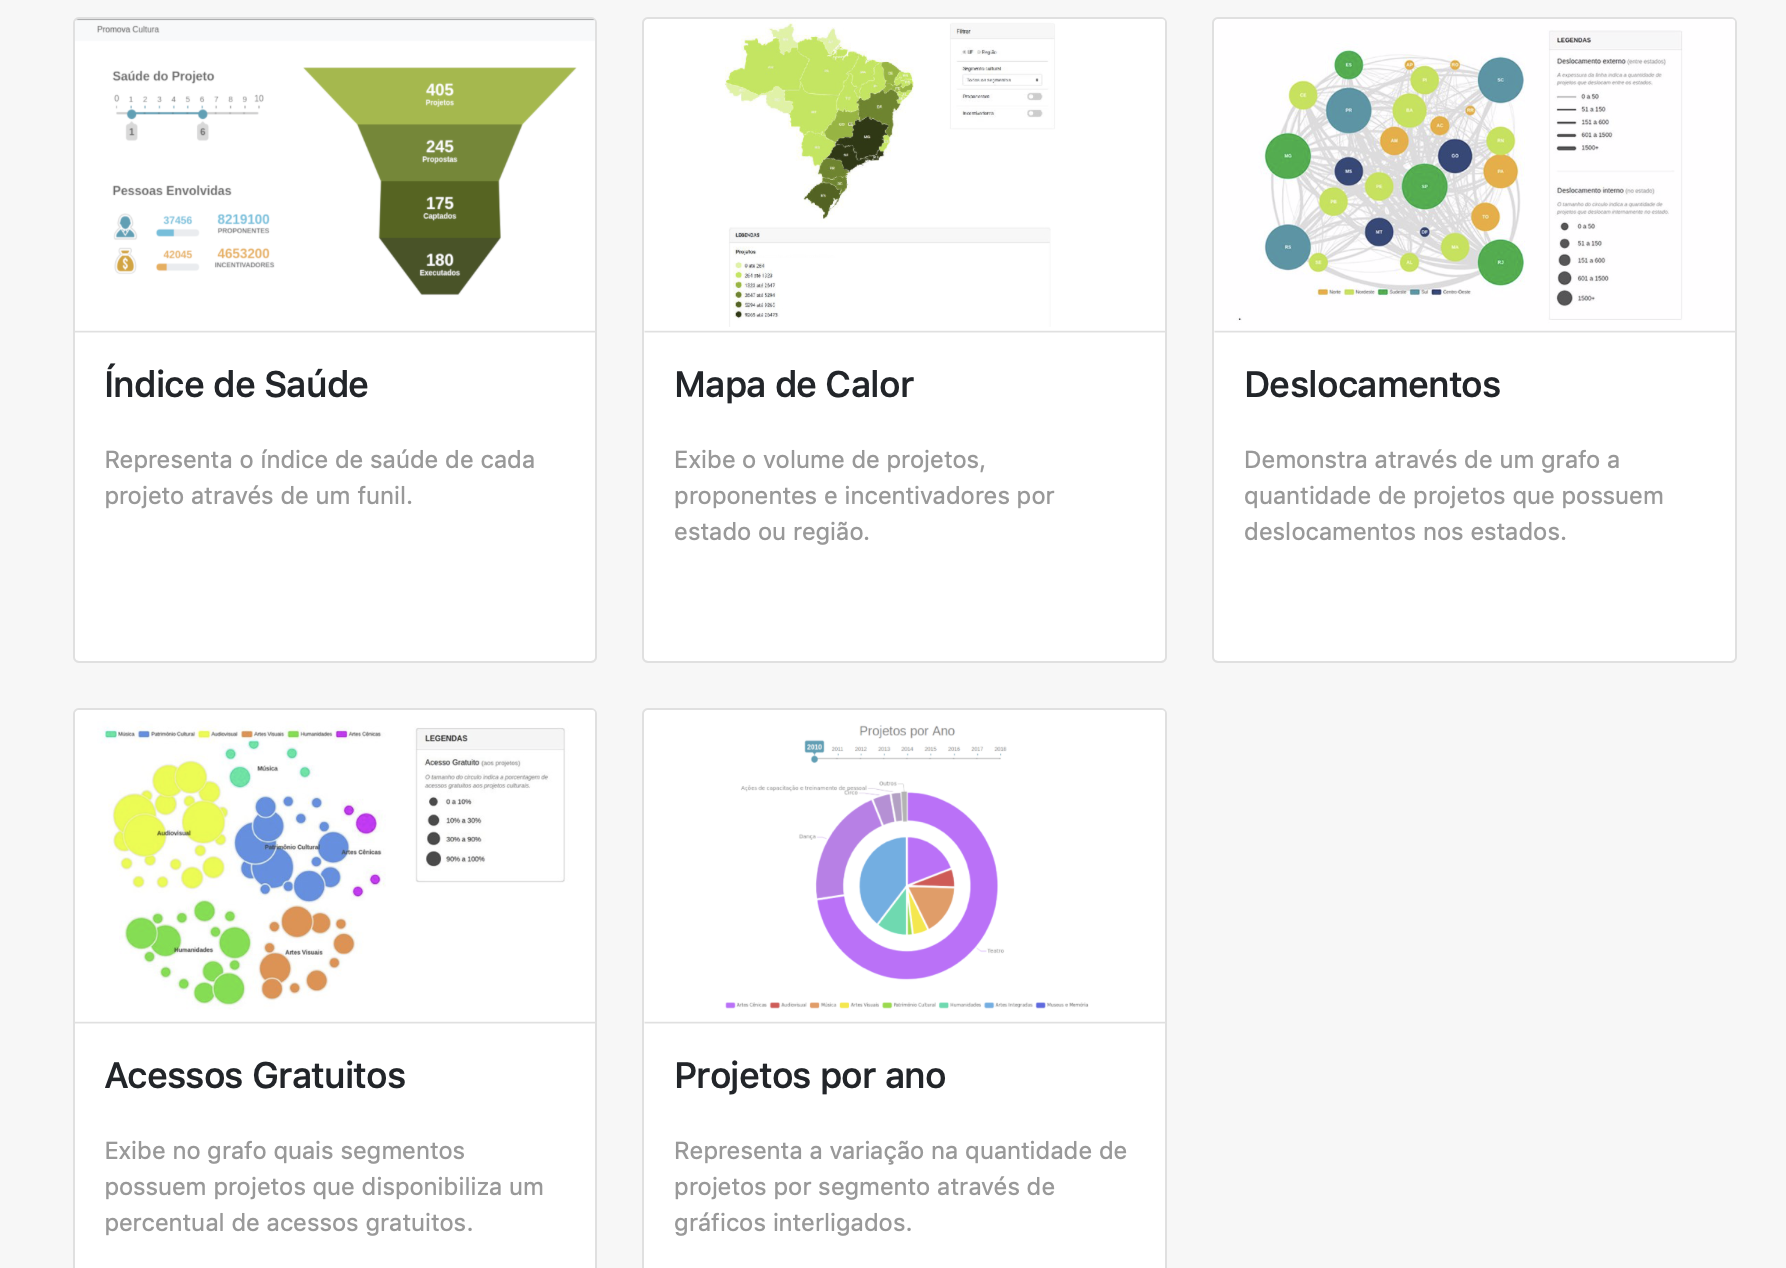
\includegraphics{https://raw.githubusercontent.com/lappis-unb/EcossistemasSWLivre/master/Relatorios/R4/figs/visualizacao.png}
\item
  \href{https://github.com/lappis-unb/EcossistemasSWLivre/tree/master/Relatorios/R4}{Relatório
  de Acompanhamento 4}
\item
  \href{http://sistemas.cultura.gov.br/comparar/salicnet/salicnet.php}{Portal
  Comparar}
\item
  \href{https://docs.google.com/spreadsheets/d/1HjrNITQ8EGYVrMCxTMUh14Ogyaxum5WVYP4jVDwki4o/edit\#gid=1949184657}{Planilha
  de comparação dos dados necessários no portal Comparar contra os dados
  disponíveis na SALIC-API}
\item
  \href{http://sistemas.cultura.gov.br/comparar/grid_Proponente_Captacao_UF/grid_Proponente_Captacao_UF.php}{Relatório
  ``Captação de recurso por UF - desde 1992''}
\item
  \href{https://github.com/lappis-unb/EcossistemasSWLivre/tree/master/Relatorios/R5}{Relatório
  de Acompanhamento 5}
\end{itemize}

\begin{enumerate}
\def\labelenumi{\arabic{enumi}.}
\setcounter{enumi}{1}
\tightlist
\item
  \textbf{Estudos sobre a apresentação visual de resultados de
  algoritmos de aprendizado de máquina e análises estatísticas}
\end{enumerate}

\textbf{Concluído} - Esse estudo foi realizado no contexto do projeto da
Tais. Foi acoplado a arquitetura a stack elastic/Kibana para a mineração
dos dados de conversa entre a Tais e o usuário. A partir dos dados em
uso, foram projetados dashboards com métricas de uso, comportamento, e
de negócio. Ao total, foram propostos 9 graficos de negócio, 5 de
compartamento do usuário, e 4 de uso/técnico. Essas métricas foram
validadas e evoluidas. Ao final do projeto, utilizamos esses dashboards
para melhorar o desempenho da Tais, acrescentar novos conhecimentos a
sua base de treinamento. Também conseguimos prever tendências e
conteúdos mais pesquisados pelo usuário.

TODO: Imagem do gráfico do dashboard da Tais

\textbf{Documentação comprobatória} - Através de uma demanda combinada
com o antigo Ministério da Cultura, atual Secretaria Especial da Cultura
do Ministério da Cidadania, foi criada uma equipe para atuar no campo de
pesquisa e desenvolvimento na área de \emph{business intelligence} (BI).
Frente de trabalho responsável por elaborar visualizações dos dados
provenientes da interação dos usuários com a Tais.

Por ser uma nova área de atuação dentro do LAPPIS, a equipe começou
pesquisando sobre quais métricas são relevantes coletar a partir da
interação do \emph{usuário vs Tais}, fornecendo dados tanto para equipe
de desenvolvimento do \emph{chatbot}, facilitando na manutenção e
evolução da Tais, e gerando dados para a equipe de negócios, comprovando
os objetivos da implementação do projeto.

Após a pesquisa sobre as métricas, um estudo teve que ser realizado
sobre quais tecnologias seriam utilizadas para armazenar e elaborar as
visualizações propostas, seguindo a cultura do laboratório de utilização
de \emph{software}. Foi então selecionado o \emph{ElasticSearch}, como
sendo a ferramenta de armazenamento de dados, que também trabalha com
buscas em tempo real e faz o armazenamento em cache das pesquisas já
realizadas. Para consumir os dados armazenados no Elastic e tratá-los
para disponbilizar em formato de visualizações, foi utilizado o
\emph{Kibana}, um dos componentes da \emph{ElasticStack}. Essa
ferramenta fornece recursos para elaboração de dashboards e
visualizações.

Subsequente a escolha das tecnologias, a equipe atuou na implementação
de todas as visualizações propostas. Foram dividas em dois grupos,
métricas de desenvolvimento e de negócio, sendo disponibilizadas
respectivamente em dois \emph{dashboards} distintos, \emph{Paloma's} e
\emph{Perfil de Usuário}.

Com a finalização da etapa de implementação, foi automatizado o processo
de importação dos \emph{dashboards} contendo as visualizações a partir
de um único comando, evitando um retrabalho e garantindo uma entrega de
excelência.

As entregas estão documentadas nos relatórios de entrega e em alguns
estudos apresentados abaixo:

\begin{itemize}
\item
  \href{https://github.com/lappis-unb/tais/wiki/Estudo-sobre-metricas-para-bots}{Estudo
  sobre métricas}
\item
  \href{https://github.com/lappis-unb/rasa-ptbr-boilerplate/blob/master/analytics/import_dashboards.py}{Automação
  do processo de importação}
\item
  \href{https://github.com/lappis-unb/tais/blob/master/README.md}{Stack
  do Elastic/Kibana}
\item
  \href{https://github.com/lappis-unb/EcossistemasSWLivre/blob/master/Relatorios/R5/RELATÓRIO\%20ETAPA\%205.pdf}{Relatório
  Etapa 5}
\item
  \href{https://github.com/lappis-unb/EcossistemasSWLivre/blob/master/Relatorios/R6/RELATÓRIO\%20ETAPA\%206.pdf}{Relatório
  Etapa 6}
\item
  \href{https://github.com/lappis-unb/EcossistemasSWLivre/blob/master/Relatorios/R7/RELATÓRIO\%20ETAPA\%207.pdf}{Relatório
  Etapa 7}
\end{itemize}

\begin{enumerate}
\def\labelenumi{\arabic{enumi}.}
\setcounter{enumi}{2}
\tightlist
\item
  \textbf{Dashboard para a visualização e análise das relações entre
  proponentes e financiadores por meio de grafos}
\end{enumerate}

\textbf{Concluído} - A parte da equipe do ``Promova Cultura'' que foi
realocada para o SALIC-ML, conforme relatado na meta 1 deste pacote de
trabalho, se juntou aos esforços de estudo das relações entre
proponentes e incentivadores por meio de grafos. O assunto é bastante
complexo pois os mesmos atores podem assumir papéis distintos em
projetos diferentes. Por exemplo, uma incentivadora de um projeto, pode
ser proponente de um outro projeto e, ao mesmo tempo, ser fornecedora
para este mesmo projeto. Além disso, existe circularidade, onde é
necessário desmembrar pessoas jurídicas em seus sócios componentes para
aí sim, analisar a relação entre eles.

Com base nas análises preliminares dos dados e nas explorações
computacionais, foram geradas propostas de visualização, documentadas as
issues 312 e 326 do repositório. Em, 02/04/2019 a equipe recebeu a
visita de um especialista da CGEE que fez uma jornada de treinamento e
co-trabalho, apontando vários pontos que precisavam ser revistos e
aprofundados. Dada essa perspectiva e a necessidade de aprofundamento do
relatório de complexidade de análise financeira dos projetos, o tópico
principal do SALIC-ML, a equipe foi realocada para garantir a qualidade
do relatório de complexidade.

Cabe frisar que os estudos computacionais de caráter exploratório foram
100\% documentados em Jupyter notebooks (em anexo), apresentando os
cálculos em associação a visualizações científicas e explicitando as
relações entre proponentes e financiadores por meio de grafos. O que
cumpre plenamente esta meta.

O material produzido, todos os estudos e esboços de visualização, foram
apresentados como parte do Relatório de Acompanhamento 6 e aprovado
pelos gestores.

\textbf{Documentação comprobatória}

\begin{itemize}
\tightlist
\item
  \href{https://github.com/lappis-unb/salic-ml/}{Repositório do
  ``SALIC-ML''}
\item
  Exemplos de estudos de grafos:
\end{itemize}

\includegraphics{https://user-images.githubusercontent.com/38992510/55029111-07993980-4fe8-11e9-8be0-54c0abb829c5.png}
\includegraphics{https://user-images.githubusercontent.com/38992510/55029348-a32aaa00-4fe8-11e9-8dc9-abf585f80618.png}
\includegraphics{https://user-images.githubusercontent.com/38992510/55029567-24823c80-4fe9-11e9-920a-545b249fdb20.png}
\includegraphics{https://user-images.githubusercontent.com/38992510/55029711-85117980-4fe9-11e9-87ac-676af291d7ac.png}
\includegraphics{https://user-images.githubusercontent.com/38992510/55029866-e9ccd400-4fe9-11e9-9d00-bf29971c8971.png}
\includegraphics{https://user-images.githubusercontent.com/38992510/55030330-eede5300-4fea-11e9-8eee-58a3ef8ffb82.png}
\includegraphics{https://user-images.githubusercontent.com/38992510/55030556-68764100-4feb-11e9-8dc5-a8c69815d69e.png}
\includegraphics{https://user-images.githubusercontent.com/38992510/55031159-ba6b9680-4fec-11e9-9a0b-614b20f3afd3.png}\\
- \href{https://github.com/lappis-unb/salic-ml/issues/312}{Issue 312} -
\href{https://github.com/lappis-unb/salic-ml/issues/326}{Issue 326} -
\href{https://github.com/lappis-unb/EcossistemasSWLivre/blob/master/Relatorios/R6/}{Relatório
de Acompanhamento 6}

\hypertarget{pacote-de-trabalho-estudos-dos-processos-tuxe9cnicos-e-gerenciais-minc-para-aferiuxe7uxe3o-e-aceitauxe7uxe3o-de-produtos-de-software}{%
\subsection{Pacote de Trabalho: Estudos dos processos técnicos e
gerenciais MinC para aferição e aceitação de produtos de
software}\label{pacote-de-trabalho-estudos-dos-processos-tuxe9cnicos-e-gerenciais-minc-para-aferiuxe7uxe3o-e-aceitauxe7uxe3o-de-produtos-de-software}}

De acordo com o plano de trabalho, "O objetivo geral desta frente de
pesquisa é auxiliar os times de desenvolvimento e gestores de TI do MinC
a aprimorarem sua capacidade em tomar decisões acerca da qualidade das
versões dos produtos de software entregues por seus fornecedores.

Esse pacote de trabalho teve seu cronograma alterado e escopo limitado.
Tais mudanças foram registradas no relatório X de acompanhamento, e
devidamente aprovados pelo ministério e universidade.

\hypertarget{metas-especuxedficas-5}{%
\subsubsection{Metas específicas}\label{metas-especuxedficas-5}}

\begin{enumerate}
\def\labelenumi{\arabic{enumi}.}
\tightlist
\item
  \textbf{Experimentação contínua aplicada a engenharia de produto de
  software}
\end{enumerate}

\textbf{Concluído} - Durante todo o projeto foi abordado a
experimentação contínua, no qual passavamos continuamento por três
etapas: (1) levantamento de hipoteses para solucionar um problema, (2)
teste de parte da solução para validar a hipótese, (3) validação da
hipótese, (4) implementação da solução no produto final. Além disso,
trabalhamos com times full-stack e orientados a produto, a fim de ter
uma qualidade alta do produto entregue. Com isso, para cada pacote de
trabalho, tinha-se um time composto por alunos de Engenharia de
Software, Designers, Alunos de letras, e profissionais plenos e seniores
para gerir os riscos de projeto.

\textbf{Documentação comprobatória}

\begin{itemize}
\item
  \href{https://github.com/lappis-unb/EcossistemasSWLivre/blob/master/Relatorios/R3/RELATÓRIO\%20ETAPA\%203.md}{Relatório
  Etapa 3}
\item
  \href{https://github.com/lappis-unb/EcossistemasSWLivre/blob/master/Relatorios/R4/RELATÓRIO\%20ETAPA\%204.pdf}{Relatório
  Etapa 4}
\end{itemize}

\begin{enumerate}
\def\labelenumi{\arabic{enumi}.}
\setcounter{enumi}{1}
\tightlist
\item
  \textbf{a mineração em repositórios de software e a análise científica
  de dados do software}
\end{enumerate}

\textbf{Concluído} - Análise que o Renato está fazendo

\textbf{Documentação comprobatória} -

\begin{enumerate}
\def\labelenumi{\arabic{enumi}.}
\setcounter{enumi}{2}
\tightlist
\item
  \textbf{prospectar uma sistemática, baseada em evidência científica,
  que auxilie a homologação de produtos de software, em obediência ao
  normativo estabelecido}
\end{enumerate}

\textbf{Concluído parcialmente} -

\textbf{Documentação comprobatória} -

\hypertarget{acompanhamento-financeiro}{%
\section{Acompanhamento Financeiro}\label{acompanhamento-financeiro}}

Tivemos completa transparência quanto ao acompanhamento financeiro do
projeto. A prestação de contas foi feita a cada relatório de
acompanhamento, no qual apresentamos não só o montante gasto, quanto
também o valor gasto por pacote de trabalho. O tamanho do time por
frente de trabalho foi definido de acordo com as prioridades
estabelecidas pelo ministério, nas reuniões estratégicas. Porém, vale
ressaltar, que por se tratar de times multidisciplinares, membros
poderiam ser alocados em diferentes frentes por diversas
\textbf{sprints} de acordo com necessidade de projeto e deadlines de
entrega.

O financeiro completo do projeto pode ser visto na figura abaixo.

\hypertarget{assinatura}{%
\section{Assinatura}\label{assinatura}}

\hypertarget{responsuxe1vel-pela-execuuxe7uxe3o}{%
\subsection{Responsável pela
Execução:}\label{responsuxe1vel-pela-execuuxe7uxe3o}}

Nome: Carla Silva Rocha Aguiar (Coordenadora do Projeto)

Assinatura:

Data:/2019

\hypertarget{anexos}{%
\section{Anexos}\label{anexos}}

\hypertarget{artigos}{%
\section{Artigos}\label{artigos}}

Artigos acadêmicos e comunicação

\hypertarget{capacitauxe7uxe3o-e-participauxe7uxe3o-em-eventos}{%
\section{Capacitação e Participação em
Eventos}\label{capacitauxe7uxe3o-e-participauxe7uxe3o-em-eventos}}

\hypertarget{documentauxe7uxe3o-tuxe9cnica-dos-projetos}{%
\section{Documentação Técnica dos
projetos}\label{documentauxe7uxe3o-tuxe9cnica-dos-projetos}}
